% $Author: oscar $
% $Date: 2013-11-27 16:48:27 +0100 (Wed, 27 Nov 2013) $
% $Revision: 35492 $
%=================================================================
\ifx\wholebook\relax\else
% --------------------------------------------
% Lulu:
	\documentclass[a4paper,10pt,twoside]{book}
	\usepackage[
		papersize={6.13in,9.21in},
		hmargin={.815in,.815in},
		vmargin={.98in,.98in},
		ignoreheadfoot
	]{geometry}
  \usepackage[hangul]{kotex}
	% $Author: oscar $
% $Date: 2009-09-13 20:58:29 +0200 (Sun, 13 Sep 2009) $
% $Revision: 29070 $
%=============================================================
% NB: documentclass must be set in main document.
% Allows book to be generated in multiple formats.
%=============================================================
%:Packages
\usepackage[T1]{fontenc}  %%%%%really important to get the code directly in the text!
\usepackage{palatino}
\usepackage{ifthen}
\usepackage{graphicx}
\graphicspath{{figures/}}
\usepackage{xspace}
\usepackage{makeidx}
\usepackage{isodateo} % enable \isodate
\usepackage{amssymb,textcomp}
%=============================================================
%:More packages
%\usepackage[english]{babel}
%\usepackage{lmodern}
%\usepackage[scaled=0.85]{helvet}
%\usepackage{microtype}
%\usepackage{theorem}
%\usepackage{float}
%\usepackage{longtable}
%\usepackage[nottoc]{tocbibind}
%\usepackage{multicol}
%\usepackage{booktabs}	% book-style tables
%\usepackage{topcapt}	% enables \topcaption
%\usepackage{multirow}
%\usepackage{tabularx}
%\usepackage{alltt}
\usepackage[usenames,dvipsnames]{color}
%\usepackage[hang]{subfigure}\makeatletter\def\p@subfigure{\thefigure\,}\makeatother
%\usepackage{rotating}
%\usepackage{enumitem}	% apb: allows more control over tags in enumerations
%\usepackage{verbatim}     % for comment environment
%\usepackage{varioref}	% for page references that work
%\usepackage{needspace}
%\usepackage[newparttoc]{titlesec}
%\usepackage{titletoc}
%\usepackage{wrapfig}
\usepackage[
	colorlinks=true,
	linkcolor=black,
	urlcolor=black,
	citecolor=black
]{hyperref}   % should come last
%=============================================================
%:URL style
\makeatletter
\def\url@leostyle{%
  \@ifundefined{selectfont}{\def\UrlFont{\sf}}{\def\UrlFont{\sffamily}}}
\makeatother
\urlstyle{leo}
%=============================================================
%:Booleans
\newboolean{lulu}
\setboolean{lulu}{false}
\newcommand{\ifluluelse}[2]{\ifthenelse{\boolean{lulu}}{#1}{#2}}
%=============================================================
%:Editorial comment macros
\newcommand{\nnbb}[2]{
  \fbox{\bfseries\sffamily\scriptsize#1}
  {\sf\small$\blacktriangleright$\textit{#2}$\blacktriangleleft$}
}
\newcommand{\on}[1]{\nnbb{Oscar}{#1}}
\newcommand{\here}{\nnbb{CONTINUE}{HERE}}
%=============================================================
%:Abbreviation macros
\newcommand{\ie}{\emph{i.e.},\xspace}
\newcommand{\eg}{\emph{e.g.},\xspace}
\newcommand{\etc}{\emph{etc.}\xspace}
\newcommand{\etal}{\emph{et al.}\xspace}
\newcommand{\straightquote}{"}
\newcommand{\sba}{\url{SquareBracketAssociates.org}\xspace}
%=============================================================
%:Patterns
% \newcommand{\pattern}[2]{\newpage\section{{\sf #1}}\label{pat:#2}}
% \newcommand{\pattern}[2]{\newpage\index{#1 (Pattern)}\section{#1}\label{pat:#2}}
\newcommand{\pattern}[2]{\cleardoublepage\index{#1 (패턴)}\section{#1}\label{pat:#2}}
\newcommand{\thumbnail}[2]{\index{#1 (패턴)}\subsection{#1}\label{pat:#2}}
\newcommand{\thumblang}[2]{\index{#1 (패턴 랭귀지)}\subsection{#1}\label{pat:#2}}
\newcommand{\variant}[1]{{\emph{#1}}\xspace}
% \newcommand{\problem}[1]{\subsection*{Problem}\emph{#1}}
\newcommand{\intent}[1]{\paragraph{의도}\emph{#1}}
\newcommand{\problem}[1]{\paragraph{문제}\emph{#1}}
\newcommand{\solution}[1]{\paragraph{해결}\emph{#1}}
\newcommand{\discussion}[0]{\paragraph{토론}}
\newcommand{\cmd}[1]{{\tt #1}\xspace}
%=============================================================
%:Environments
\newenvironment{bulletlist}{\begin{itemize}\setlength{\itemsep}{0ex}}
{\end{itemize}}
%=============================================================
%:Cross reference macros
\newcommand{\chalabel}[1]{\label{cha:#1}}
\newcommand{\seclabel}[1]{\label{sec:#1}}
\newcommand{\figlabel}[1]{\label{fig:#1}}
\newcommand{\tablabel}[1]{\label{tab:#1}}
\newcommand{\rulelabel}[1]{\label{rule:#1}}
\newcommand{\eglabel}[1]{\label{eg:#1}}
\newcommand{\scrlabel}[1]{\label{scr:#1}}
\newcommand{\mthlabel}[1]{\label{mth:#1}}
\newcommand{\clslabel}[1]{\label{cls:#1}}
\newcommand{\faqlabel}[1]{\label{faq:#1}}
%\newcommand{\charef}[1]{Chapter~\ref{cha:#1}\xspace}
%\newcommand{\secref}[1]{Section~\ref{sec:#1}\xspace}
\newcommand{\figref}[1]{Figure~\ref{fig:#1}\xspace}
% \newcommand{\patpgref}[2]{\hyperref[pat:#2]{\sf #1} [p.~\pageref{pat:#2}]\xspace}
\newcommand{\patpgref}[2]{\index{#1 (Pattern)}\hyperref[pat:#2]{#1} [p.~\pageref{pat:#2}]\xspace}
\newcommand{\patlangpgref}[2]{\index{#1 (Pattern language)}\hyperref[pat:#2]{#1} [p.~\pageref{pat:#2}]\xspace}
% \newcommand{\patref}[2]{\hyperref[pat:#2]{\sf #1}\xspace}
\newcommand{\patref}[2]{\index{#1 (Pattern)}\hyperref[pat:#2]{#1}\xspace}
\newcommand{\patlangref}[2]{\index{#1 (Pattern language)}\hyperref[pat:#2]{#1}\xspace}
% \newcommand{\charef}[2]{\hyperref[cha:#2]{\underline{\sf #1}}\xspace}
% \newcommand{\charef}[2]{\hyperref[cha:#2]{\sf #1}\xspace}
\newcommand{\charef}[2]{\index{#1 (Pattern cluster)}\hyperref[cha:#2]{#1}\xspace}
% \newcommand{\chapgref}[2]{\hyperref[cha:#2]{\sf #1} [p.~\pageref{cha:#2}]\xspace}
\newcommand{\chapgref}[2]{\index{#1 (Pattern cluster)}\hyperref[cha:#2]{#1} [p.~\pageref{cha:#2}]\xspace}
%\newcommand{\Figref}[1]{Figure~\ref{fig:#1}\xspace}
%\newcommand{\appref}[1]{Appendix~\ref{app:#1}\xspace}
%\newcommand{\tabref}[1]{Table~\ref{tab:#1}\xspace}
%\newcommand{\ruleref}[1]{\ref{rule:#1}\xspace}
%\newcommand{\egref}[1]{example~\ref{eg:#1}\xspace}
%\newcommand{\Egref}[1]{Example~\ref{eg:#1}\xspace}
%\newcommand{\scrref}[1]{script~\ref{scr:#1}\xspace}
%\newcommand{\Scrref}[1]{Script~\ref{scr:#1}\xspace}
%\newcommand{\tscrref}[1]{the script~\ref{scr:#1}\xspace}
%\newcommand{\Tscrref}[1]{The script~\ref{scr:#1}\xspace}
%\newcommand{\mthref}[1]{method~\ref{mth:#1}\xspace}
%\newcommand{\mthsref}[1]{methods~\ref{mth:#1}\xspace}
%\newcommand{\Mthref}[1]{Method~\ref{mth:#1}\xspace}
%\newcommand{\tmthref}[1]{the method~\ref{mth:#1}\xspace}
%\newcommand{\Tmthref}[1]{The method~\ref{mth:#1}\xspace}
%\newcommand{\clsref}[1]{class~\ref{cls:#1}\xspace}
%\newcommand{\tclsref}[1]{the class~\ref{cls:#1}\xspace}
%\newcommand{\Tclsref}[1]{The class~\ref{cls:#1}\xspace}
%=============================================================
%:Page Layout
\setlength{\headsep}{1cm}
%=============================================================
%:Menu item macro
%\definecolor{lightgray}{gray}{0.89}
%\newcommand{\menu}[1]{{%
%	\setlength{\fboxsep}{0pt}%
%	\colorbox{lightgray}{{{\upshape\sffamily\strut \,#1\,}}}}}
%\newcommand{\go}{\,$\triangleright$\,}
%\newcommand{\short}[1]{\mbox{{\sc cmd}\hspace{0.08em}--\hspace{0.09em}#1}\xspace}
%\newcommand{\button}[1]{{%
%	\setlength{\fboxsep}{0pt}%
%	\fbox{{\upshape\sffamily\strut \,#1\,}}}}
%\newcommand{\toolsflap}{\textit{Tools} flap\xspace}
%=============================================================
%:Section depth
%\setcounter{secnumdepth}{2}
%
%\DeclareGraphicsExtensions{.pdf, .jpg, .png}
%=============================================================
%:PDF setup
\hypersetup{
   pdftitle={Object-Oriented Reengineering Patterns},
   pdfauthor={Serge Demeyer, St\'ephane Ducasse, Oscar Nierstrasz},
   pdfkeywords={Reengineering, Object-Oriented Programming, Patterns},
   pdfsubject={Computer Science}
}
%=============================================================
%:Page layout and appearance
%\renewcommand{\chaptermark}[1]{\markboth{#1}{}}
%\renewcommand{\sectionmark}[1]{\markright{\thesection\ #1}}
%\renewpagestyle{plain}[\small\itshape]{%
%	\setheadrule{0pt}%
%	\sethead[][][]{}{}{}%
%	\setfoot[][][]{}{}{}}
%\renewpagestyle{headings}[\small\itshape]{%
%	\setheadrule{0pt}%
%	\setmarks{chapter}{section}%
%	\sethead[\thepage][][\chaptertitle]{\sectiontitle}{}{\thepage}%
%	\setfoot[][][]{}{}{}}
%=============================================================
%:Title section setup and TOC numbering depth
%\setcounter{secnumdepth}{1}
%\setcounter{tocdepth}{1}
%\titleformat{\part}[display]{\centering}{\huge\partname\ \thepart}{1em}{\Huge\textbf}[]
%\titleformat{\chapter}[display]{}{\huge\chaptertitlename\ \thechapter}{1em}{\Huge\raggedright\textbf}[]
%\titlecontents{part}[3pc]{%
%		\pagebreak[2]\addvspace{1em plus.4em minus.2em}%
%		\leavevmode\large\bfseries}
%	{\contentslabel{3pc}}{\hspace*{-3pc}}
%	{}[\nopagebreak]
%\titlecontents{chapter}[3pc]{%
%		\pagebreak[0]\addvspace{1em plus.2em minus.2em}%
%		\leavevmode\bfseries}
%	{\contentslabel{3pc}}{}
%	{\hfill\contentspage}[\nopagebreak]
%\dottedcontents{section}[3pc]{}{3pc}{1pc}
%\dottedcontents{subsection}[3pc]{}{0pc}{1pc}
%\let\origdoublepage\cleardoublepage
%\newcommand{\clearemptydoublepage}{%
%  \clearpage
%  {\pagestyle{empty}\origdoublepage}}
%\let\cleardoublepage\clearemptydoublepage % see http://www.tex.ac.uk/cgi-bin/texfaq2html?label=patch
%=============================================================
%:Listings package configuration
\newcommand{\caret}{\makebox{\raisebox{0.4ex}{\footnotesize{$\wedge$}}}}
% \newcommand{\escape}{{\sf \textbackslash}}
\definecolor{source}{gray}{0.95}
\usepackage{listings}
\lstdefinelanguage{Smalltalk}{
  morestring=[d]',
% Adapt this to other languages!
%  morecomment=[s]{"}{"},
  alsoletter={\#:},
  %escapechar={!},
  literate=
    {BANG}{!}1
%    {UNDERSCORE}{\_}1
    {\\st}{Smalltalk}9 % convenience -- in case \st occurs in code
    % {'}{{\textquotesingle}}1 % replaced by upquote=true in \lstset
%    {_}{{$\leftarrow$}}1
    {>>>}{{\sep}}1
    {^}{{$\uparrow$}}1
    {~}{{$\sim$}}1
    {-}{{\sf -\hspace{-0.13em}-}}1  % the goal is to make - the same width as +
    {+}{\raisebox{0.08ex}{+}}1		% and to raise + off the baseline to match -
    {-->}{{\quad$\longrightarrow$\quad}}3
	, % Don't forget the comma at the end!
  tabsize=4
}[keywords,comments,strings]

\lstset{language=Smalltalk,
	basicstyle=\sffamily,
	keywordstyle=\color{black}\bfseries,
	% stringstyle=\ttfamily, % Ugly! do we really want this? -- on
	mathescape=true,
	showstringspaces=false,
	keepspaces=true,
	breaklines=true,
	breakautoindent=true,
	backgroundcolor=\color{source},
	lineskip={-1pt}, % Ugly hack
	upquote=true, % straight quote; requires textcomp package
	columns=fullflexible} % no fixed width fonts
% \newcommand{\ct}{\lstinline[mathescape=false,basicstyle={\sffamily\upshape}]}
\newcommand{\ct}{\lstinline[mathescape=false,backgroundcolor=\color{white},basicstyle={\sffamily\upshape}]}
\newcommand{\lct}[1]{{\textsf{\textup{#1}}}}
%\newcommand{\scat}[1]{\emph{\textsf{#1}}\xspace}
%\newcommand{\prot}[1]{\emph{\textsf{#1}}\xspace}
% NB: No argument!
\lstnewenvironment{code}[0]{%
	\lstset{%
		% frame=lines,
		frame=single,
		framerule=0pt,
		mathescape=false
	}
}{}
%\def\ignoredollar#1{}
%=============================================================
%:Reserving space
%\newcommand{\needlines}[1]{\Needspace{#1\baselineskip}}
%=============================================================
%:Indexing macros
% Macros ending with "ind" generate text as well as an index entry
% Macros ending with "index" *only* generate an index entry
\newcommand{\ind}[1]{\index{#1}#1\xspace} % plain text
\newcommand{\subind}[2]{\index{#1!#2}#2\xspace} % show #2, subindex under #1
\newcommand{\emphind}[1]{\index{#1}\emph{#1}\xspace} % emph #1
\newcommand{\emphsubind}[2]{\index{#1!#2}\emph{#2}\xspace} % show emph #2, subindex under #1
\newcommand{\patind}[1]{\index{#1@#1 (pattern)}\ct{#1}\xspace} % pattern
\newcommand{\seeindex}[2]{\index{#1|see{#2}}} % #1, see #2
%\newcommand{\boldidx}[1]{{\bf #1}} % breaks hyperlink
%\newcommand{\indmain}[1]{\index{#1}#1\xspace} 
%\newcommand{\emphsubindmain}[2]{\index{#1!#2}\emph{#2}\xspace} % subindex, main entry
%\newcommand{\subindmain}[2]{\index{#1!#2}#2\xspace} % subindex, main entry
%\newcommand{\clsindmain}[1]{\index{#1!\#@(class)}\ct{#1}\xspace} % class main
%\newcommand{\indexmain}[1]{\index{#1}} 
%=============================================================
\parskip 1ex
%=============================================================

	\pagestyle{headings}
	\setboolean{lulu}{true}
% --------------------------------------------
% A4:
%	\documentclass[a4paper,11pt,twoside]{book}
%	% $Author: oscar $
% $Date: 2009-09-13 20:58:29 +0200 (Sun, 13 Sep 2009) $
% $Revision: 29070 $
%=============================================================
% NB: documentclass must be set in main document.
% Allows book to be generated in multiple formats.
%=============================================================
%:Packages
\usepackage[T1]{fontenc}  %%%%%really important to get the code directly in the text!
\usepackage{palatino}
\usepackage{ifthen}
\usepackage{graphicx}
\graphicspath{{figures/}}
\usepackage{xspace}
\usepackage{makeidx}
\usepackage{isodateo} % enable \isodate
\usepackage{amssymb,textcomp}
%=============================================================
%:More packages
%\usepackage[english]{babel}
%\usepackage{lmodern}
%\usepackage[scaled=0.85]{helvet}
%\usepackage{microtype}
%\usepackage{theorem}
%\usepackage{float}
%\usepackage{longtable}
%\usepackage[nottoc]{tocbibind}
%\usepackage{multicol}
%\usepackage{booktabs}	% book-style tables
%\usepackage{topcapt}	% enables \topcaption
%\usepackage{multirow}
%\usepackage{tabularx}
%\usepackage{alltt}
\usepackage[usenames,dvipsnames]{color}
%\usepackage[hang]{subfigure}\makeatletter\def\p@subfigure{\thefigure\,}\makeatother
%\usepackage{rotating}
%\usepackage{enumitem}	% apb: allows more control over tags in enumerations
%\usepackage{verbatim}     % for comment environment
%\usepackage{varioref}	% for page references that work
%\usepackage{needspace}
%\usepackage[newparttoc]{titlesec}
%\usepackage{titletoc}
%\usepackage{wrapfig}
\usepackage[
	colorlinks=true,
	linkcolor=black,
	urlcolor=black,
	citecolor=black
]{hyperref}   % should come last
%=============================================================
%:URL style
\makeatletter
\def\url@leostyle{%
  \@ifundefined{selectfont}{\def\UrlFont{\sf}}{\def\UrlFont{\sffamily}}}
\makeatother
\urlstyle{leo}
%=============================================================
%:Booleans
\newboolean{lulu}
\setboolean{lulu}{false}
\newcommand{\ifluluelse}[2]{\ifthenelse{\boolean{lulu}}{#1}{#2}}
%=============================================================
%:Editorial comment macros
\newcommand{\nnbb}[2]{
  \fbox{\bfseries\sffamily\scriptsize#1}
  {\sf\small$\blacktriangleright$\textit{#2}$\blacktriangleleft$}
}
\newcommand{\on}[1]{\nnbb{Oscar}{#1}}
\newcommand{\here}{\nnbb{CONTINUE}{HERE}}
%=============================================================
%:Abbreviation macros
\newcommand{\ie}{\emph{i.e.},\xspace}
\newcommand{\eg}{\emph{e.g.},\xspace}
\newcommand{\etc}{\emph{etc.}\xspace}
\newcommand{\etal}{\emph{et al.}\xspace}
\newcommand{\straightquote}{"}
\newcommand{\sba}{\url{SquareBracketAssociates.org}\xspace}
%=============================================================
%:Patterns
% \newcommand{\pattern}[2]{\newpage\section{{\sf #1}}\label{pat:#2}}
% \newcommand{\pattern}[2]{\newpage\index{#1 (Pattern)}\section{#1}\label{pat:#2}}
\newcommand{\pattern}[2]{\cleardoublepage\index{#1 (패턴)}\section{#1}\label{pat:#2}}
\newcommand{\thumbnail}[2]{\index{#1 (패턴)}\subsection{#1}\label{pat:#2}}
\newcommand{\thumblang}[2]{\index{#1 (패턴 랭귀지)}\subsection{#1}\label{pat:#2}}
\newcommand{\variant}[1]{{\emph{#1}}\xspace}
% \newcommand{\problem}[1]{\subsection*{Problem}\emph{#1}}
\newcommand{\intent}[1]{\paragraph{의도}\emph{#1}}
\newcommand{\problem}[1]{\paragraph{문제}\emph{#1}}
\newcommand{\solution}[1]{\paragraph{해결}\emph{#1}}
\newcommand{\discussion}[0]{\paragraph{토론}}
\newcommand{\cmd}[1]{{\tt #1}\xspace}
%=============================================================
%:Environments
\newenvironment{bulletlist}{\begin{itemize}\setlength{\itemsep}{0ex}}
{\end{itemize}}
%=============================================================
%:Cross reference macros
\newcommand{\chalabel}[1]{\label{cha:#1}}
\newcommand{\seclabel}[1]{\label{sec:#1}}
\newcommand{\figlabel}[1]{\label{fig:#1}}
\newcommand{\tablabel}[1]{\label{tab:#1}}
\newcommand{\rulelabel}[1]{\label{rule:#1}}
\newcommand{\eglabel}[1]{\label{eg:#1}}
\newcommand{\scrlabel}[1]{\label{scr:#1}}
\newcommand{\mthlabel}[1]{\label{mth:#1}}
\newcommand{\clslabel}[1]{\label{cls:#1}}
\newcommand{\faqlabel}[1]{\label{faq:#1}}
%\newcommand{\charef}[1]{Chapter~\ref{cha:#1}\xspace}
%\newcommand{\secref}[1]{Section~\ref{sec:#1}\xspace}
\newcommand{\figref}[1]{Figure~\ref{fig:#1}\xspace}
% \newcommand{\patpgref}[2]{\hyperref[pat:#2]{\sf #1} [p.~\pageref{pat:#2}]\xspace}
\newcommand{\patpgref}[2]{\index{#1 (Pattern)}\hyperref[pat:#2]{#1} [p.~\pageref{pat:#2}]\xspace}
\newcommand{\patlangpgref}[2]{\index{#1 (Pattern language)}\hyperref[pat:#2]{#1} [p.~\pageref{pat:#2}]\xspace}
% \newcommand{\patref}[2]{\hyperref[pat:#2]{\sf #1}\xspace}
\newcommand{\patref}[2]{\index{#1 (Pattern)}\hyperref[pat:#2]{#1}\xspace}
\newcommand{\patlangref}[2]{\index{#1 (Pattern language)}\hyperref[pat:#2]{#1}\xspace}
% \newcommand{\charef}[2]{\hyperref[cha:#2]{\underline{\sf #1}}\xspace}
% \newcommand{\charef}[2]{\hyperref[cha:#2]{\sf #1}\xspace}
\newcommand{\charef}[2]{\index{#1 (Pattern cluster)}\hyperref[cha:#2]{#1}\xspace}
% \newcommand{\chapgref}[2]{\hyperref[cha:#2]{\sf #1} [p.~\pageref{cha:#2}]\xspace}
\newcommand{\chapgref}[2]{\index{#1 (Pattern cluster)}\hyperref[cha:#2]{#1} [p.~\pageref{cha:#2}]\xspace}
%\newcommand{\Figref}[1]{Figure~\ref{fig:#1}\xspace}
%\newcommand{\appref}[1]{Appendix~\ref{app:#1}\xspace}
%\newcommand{\tabref}[1]{Table~\ref{tab:#1}\xspace}
%\newcommand{\ruleref}[1]{\ref{rule:#1}\xspace}
%\newcommand{\egref}[1]{example~\ref{eg:#1}\xspace}
%\newcommand{\Egref}[1]{Example~\ref{eg:#1}\xspace}
%\newcommand{\scrref}[1]{script~\ref{scr:#1}\xspace}
%\newcommand{\Scrref}[1]{Script~\ref{scr:#1}\xspace}
%\newcommand{\tscrref}[1]{the script~\ref{scr:#1}\xspace}
%\newcommand{\Tscrref}[1]{The script~\ref{scr:#1}\xspace}
%\newcommand{\mthref}[1]{method~\ref{mth:#1}\xspace}
%\newcommand{\mthsref}[1]{methods~\ref{mth:#1}\xspace}
%\newcommand{\Mthref}[1]{Method~\ref{mth:#1}\xspace}
%\newcommand{\tmthref}[1]{the method~\ref{mth:#1}\xspace}
%\newcommand{\Tmthref}[1]{The method~\ref{mth:#1}\xspace}
%\newcommand{\clsref}[1]{class~\ref{cls:#1}\xspace}
%\newcommand{\tclsref}[1]{the class~\ref{cls:#1}\xspace}
%\newcommand{\Tclsref}[1]{The class~\ref{cls:#1}\xspace}
%=============================================================
%:Page Layout
\setlength{\headsep}{1cm}
%=============================================================
%:Menu item macro
%\definecolor{lightgray}{gray}{0.89}
%\newcommand{\menu}[1]{{%
%	\setlength{\fboxsep}{0pt}%
%	\colorbox{lightgray}{{{\upshape\sffamily\strut \,#1\,}}}}}
%\newcommand{\go}{\,$\triangleright$\,}
%\newcommand{\short}[1]{\mbox{{\sc cmd}\hspace{0.08em}--\hspace{0.09em}#1}\xspace}
%\newcommand{\button}[1]{{%
%	\setlength{\fboxsep}{0pt}%
%	\fbox{{\upshape\sffamily\strut \,#1\,}}}}
%\newcommand{\toolsflap}{\textit{Tools} flap\xspace}
%=============================================================
%:Section depth
%\setcounter{secnumdepth}{2}
%
%\DeclareGraphicsExtensions{.pdf, .jpg, .png}
%=============================================================
%:PDF setup
\hypersetup{
   pdftitle={Object-Oriented Reengineering Patterns},
   pdfauthor={Serge Demeyer, St\'ephane Ducasse, Oscar Nierstrasz},
   pdfkeywords={Reengineering, Object-Oriented Programming, Patterns},
   pdfsubject={Computer Science}
}
%=============================================================
%:Page layout and appearance
%\renewcommand{\chaptermark}[1]{\markboth{#1}{}}
%\renewcommand{\sectionmark}[1]{\markright{\thesection\ #1}}
%\renewpagestyle{plain}[\small\itshape]{%
%	\setheadrule{0pt}%
%	\sethead[][][]{}{}{}%
%	\setfoot[][][]{}{}{}}
%\renewpagestyle{headings}[\small\itshape]{%
%	\setheadrule{0pt}%
%	\setmarks{chapter}{section}%
%	\sethead[\thepage][][\chaptertitle]{\sectiontitle}{}{\thepage}%
%	\setfoot[][][]{}{}{}}
%=============================================================
%:Title section setup and TOC numbering depth
%\setcounter{secnumdepth}{1}
%\setcounter{tocdepth}{1}
%\titleformat{\part}[display]{\centering}{\huge\partname\ \thepart}{1em}{\Huge\textbf}[]
%\titleformat{\chapter}[display]{}{\huge\chaptertitlename\ \thechapter}{1em}{\Huge\raggedright\textbf}[]
%\titlecontents{part}[3pc]{%
%		\pagebreak[2]\addvspace{1em plus.4em minus.2em}%
%		\leavevmode\large\bfseries}
%	{\contentslabel{3pc}}{\hspace*{-3pc}}
%	{}[\nopagebreak]
%\titlecontents{chapter}[3pc]{%
%		\pagebreak[0]\addvspace{1em plus.2em minus.2em}%
%		\leavevmode\bfseries}
%	{\contentslabel{3pc}}{}
%	{\hfill\contentspage}[\nopagebreak]
%\dottedcontents{section}[3pc]{}{3pc}{1pc}
%\dottedcontents{subsection}[3pc]{}{0pc}{1pc}
%\let\origdoublepage\cleardoublepage
%\newcommand{\clearemptydoublepage}{%
%  \clearpage
%  {\pagestyle{empty}\origdoublepage}}
%\let\cleardoublepage\clearemptydoublepage % see http://www.tex.ac.uk/cgi-bin/texfaq2html?label=patch
%=============================================================
%:Listings package configuration
\newcommand{\caret}{\makebox{\raisebox{0.4ex}{\footnotesize{$\wedge$}}}}
% \newcommand{\escape}{{\sf \textbackslash}}
\definecolor{source}{gray}{0.95}
\usepackage{listings}
\lstdefinelanguage{Smalltalk}{
  morestring=[d]',
% Adapt this to other languages!
%  morecomment=[s]{"}{"},
  alsoletter={\#:},
  %escapechar={!},
  literate=
    {BANG}{!}1
%    {UNDERSCORE}{\_}1
    {\\st}{Smalltalk}9 % convenience -- in case \st occurs in code
    % {'}{{\textquotesingle}}1 % replaced by upquote=true in \lstset
%    {_}{{$\leftarrow$}}1
    {>>>}{{\sep}}1
    {^}{{$\uparrow$}}1
    {~}{{$\sim$}}1
    {-}{{\sf -\hspace{-0.13em}-}}1  % the goal is to make - the same width as +
    {+}{\raisebox{0.08ex}{+}}1		% and to raise + off the baseline to match -
    {-->}{{\quad$\longrightarrow$\quad}}3
	, % Don't forget the comma at the end!
  tabsize=4
}[keywords,comments,strings]

\lstset{language=Smalltalk,
	basicstyle=\sffamily,
	keywordstyle=\color{black}\bfseries,
	% stringstyle=\ttfamily, % Ugly! do we really want this? -- on
	mathescape=true,
	showstringspaces=false,
	keepspaces=true,
	breaklines=true,
	breakautoindent=true,
	backgroundcolor=\color{source},
	lineskip={-1pt}, % Ugly hack
	upquote=true, % straight quote; requires textcomp package
	columns=fullflexible} % no fixed width fonts
% \newcommand{\ct}{\lstinline[mathescape=false,basicstyle={\sffamily\upshape}]}
\newcommand{\ct}{\lstinline[mathescape=false,backgroundcolor=\color{white},basicstyle={\sffamily\upshape}]}
\newcommand{\lct}[1]{{\textsf{\textup{#1}}}}
%\newcommand{\scat}[1]{\emph{\textsf{#1}}\xspace}
%\newcommand{\prot}[1]{\emph{\textsf{#1}}\xspace}
% NB: No argument!
\lstnewenvironment{code}[0]{%
	\lstset{%
		% frame=lines,
		frame=single,
		framerule=0pt,
		mathescape=false
	}
}{}
%\def\ignoredollar#1{}
%=============================================================
%:Reserving space
%\newcommand{\needlines}[1]{\Needspace{#1\baselineskip}}
%=============================================================
%:Indexing macros
% Macros ending with "ind" generate text as well as an index entry
% Macros ending with "index" *only* generate an index entry
\newcommand{\ind}[1]{\index{#1}#1\xspace} % plain text
\newcommand{\subind}[2]{\index{#1!#2}#2\xspace} % show #2, subindex under #1
\newcommand{\emphind}[1]{\index{#1}\emph{#1}\xspace} % emph #1
\newcommand{\emphsubind}[2]{\index{#1!#2}\emph{#2}\xspace} % show emph #2, subindex under #1
\newcommand{\patind}[1]{\index{#1@#1 (pattern)}\ct{#1}\xspace} % pattern
\newcommand{\seeindex}[2]{\index{#1|see{#2}}} % #1, see #2
%\newcommand{\boldidx}[1]{{\bf #1}} % breaks hyperlink
%\newcommand{\indmain}[1]{\index{#1}#1\xspace} 
%\newcommand{\emphsubindmain}[2]{\index{#1!#2}\emph{#2}\xspace} % subindex, main entry
%\newcommand{\subindmain}[2]{\index{#1!#2}#2\xspace} % subindex, main entry
%\newcommand{\clsindmain}[1]{\index{#1!\#@(class)}\ct{#1}\xspace} % class main
%\newcommand{\indexmain}[1]{\index{#1}} 
%=============================================================
\parskip 1ex
%=============================================================

%	\usepackage{a4wide}
% --------------------------------------------
	\begin{document}
	\renewcommand{\nnbb}[2]{} % Disable editorial comments
	\sloppy
\fi
%=================================================================
\chapter{초기 이해}
\chalabel{InitialUnderstanding}

여러분의 회사는 의사들이 사용할 수 있는 \emph{proDoc}이라는 의료 정보 시스템을 개발하여 제공하고 있다. 이제 회사는 다양한 의료 보험 회사와 거래를 수행하기 위해 인터넷 지원을 제공하는 경쟁 소프트웨어 \emph{XDoctor} 제품을 인수했다. 두 제품을 하나의 시스템으로 통합해야 한다.

\emph{XDoctor}를 처음 평가한 결과, 몇 가지 컴포넌트를 복구하여 통합해야 한다는 사실이 밝혀졌다. 물론 소프트웨어 컴포넌트를 성공적으로 복구하려면 내부 구조와 나머지 시스템과의 연결을 이해해야 한다. 예를 들어, 여러분의 회사는 고객에게 ``단 1바이트의 데이터도 손실되지 않는다''고 약속했으므로 데이터베이스 내용을 복구하고 결과적으로 데이터베이스 구조와 상위 계층이 데이터베이스에 어떻게 의존하는지 이해해야 한다. 또한 귀사는 건강 보험 회사와의 거래 지원을 지속하고 확대하겠다고 약속했으므로 이러한 원격 서비스와 통신하는 데 사용되는 네트워크 통신 컴포넌트를 복구해야 한다.

\subsection*{포스: 주요한 요구사항}

리엔지니어링 프로젝트에서 이와 유사한 상황이 자주 발생한다. 시스템 및 사용자와의 \chapgref{첫 번째 접근}{FirstContact}을 통해 어떤 기능이 가치가 있고 왜 복구해야 하는지 명확하게 알 수 있다. 하지만 소프트웨어 시스템의 전반적인 설계에 대한 지식이 부족하기 때문에 이 기능을 레거시 시스템에서 제거할 수 있는지 여부와 이에 소요되는 비용을 예측할 수 없다. 이러한 초기 이해는 리엔지니어링 프로젝트의 성공을 위해 매우 중요하며, 이 장에서는 이를 얻는 방법을 설명한다.

\charef{첫 번째 접근}{FirstContact}의 패턴을 통해 소프트웨어 시스템에 대한 첫 번째 아이디어를 얻는 데 도움이 되었을 것이다. 이제 이러한 아이디어를 초기 이해로 구체화하고 추가 리버스 엔지니어링 활동을 지원하기 위해 이러한 이해를 문서화할 때이다. 리버스 엔지니어링의 이 단계에서 가장 중요한 우선 순위는 나머지 프로젝트의 안정적인 기반을 구축하는 것이므로 발견한 내용이 정확하고 적절하게 문서화되어 있는지 확인해야 한다.

발견한 내용을 올바르게 문서화하는 방법은 프로젝트의 범위와 팀의 규모에 따라 크게 달라진다. 10명 이상의 개발자가 참여하는 복잡한 리버스 엔지니어링 프로젝트에는 몇 가지 표준 문서 템플릿과 구성 관리 시스템이 필요하다. 반면에 3인 미만이 참여하는 평범한 프로젝트는 중앙 서버에서 공유되는 느슨한 구조의 파일로 충분히 관리할 수 있다. 하지만 모든 상황에 적용되는 몇 가지 내재적인 포스(force)이 있다.

\begin{bulletlist}
\item \emph{데이터는 기만적이다.}
기존 소프트웨어 시스템을 이해하려면 데이터를 수집하고 해석하여 일관된 시각으로 요약해야 한다. 일반적으로 데이터를 해석하는 방법에는 두 가지 이상의 방법이 있으며, 대안 중에서 선택할 때 항상 구체적인 증거가 뒷받침되지 않는 가정을 하게 된다. \emph{따라서 정보의 출처를 다시 확인하여 탄탄한 토대 위에 이해를 구축해야 한다.}

\item \emph{이해는 반복이 필요하다.}
이해는 인간의 두뇌 내부에서 일어나므로 일종의 학습 과정에 해당하다. 리버스 엔지니어링 기술은 우리의 두뇌가 새로운 아이디어를 받아들이는 방식을 지원해야 하므로 매우 유연해야 하고 많은 반복과 역추적(backtracking)을 허용해야 한다. \emph{따라서 학습 과정을 자극하기 위해 반복(iteration)과 피드백 루프(feedback loop)를 계획해야 한다.}

\item \emph{지식을 공유해야 한다.}
시스템을 이해했다면 이 지식을 동료들과 공유하는 것이 중요하다. 동료가 업무를 수행하는 데 도움이 될 뿐만 아니라 여러분의 이해도를 높일 수 있는 의견과 피드백도 얻을 수 있다. \emph{따라서 벽에 지도를 붙이자.} 발견한 내용을 잘 보이는 곳에 게시하고 피드백에 대한 명시적인 규정을 마련하자. 이를 수행하는 방법은 팀 조직과 업무 습관에 따라 달라진다. 일반적으로 팀 회의는 정보를 공유하는 좋은 방법이지만(\patpgref{원탁 회의에 말하기}{SpeakToTheRoundTable} 참조), 커피 머신 근처의 벽에 큰 그림을 붙이는 것도 좋은 방법일 수 있다.

\item \emph{팀은 소통이 필요하다.}
시스템에 대한 이해를 구축하고 문서화하는 것은 목표가 아니라 목표를 달성하기 위한 수단이다. 시스템을 이해하기 위한 진정한 목표는 프로젝트에 참여하는 다른 사람들과 효과적으로 소통하는 것이므로, 이해한 것을 문서화하는 방식은 그 목표를 뒷받침해야 한다. 예를 들어 동료가 엔터티 관계 다이어그램(Entity-Relationship diagram)을 읽을 줄만 안다면 UML 클래스 다이어그램을 그릴 필요가 없고, 최종 사용자가 그 범위를 이해할 수 없다면 사용 사례를 작성하는 것도 의미가 없다. \emph{결국, 팀원이 사용하는 언어를 사용하자.} 팀원들이 여러분이 문서화한 내용을 읽고, 이해하고, 댓글을 달 수 있도록 여러분이 이해한 내용을 문서화할 언어를 선택하자.
\end{bulletlist}

\subsection*{개요}

소프트웨어 시스템을 처음 이해할 때 가장 우려되는 것은 잘못된 정보이다. 따라서 이러한 패턴은 신뢰할 수 있는 유일한 정보 소스인 소스 코드에 주로 의존한다.

원칙적으로 소스 코드를 연구하는 방법에는 하향식(top-down)과 상향식(bottom-up)의 두 가지 접근 방식이 있다. 실제로 모든 리버스 엔지니어링 접근 방식은 이 두 가지를 조금씩 모두 사용해야 하지만, 그래도 구분할 가치가 있다. 하향식 접근 방식에서는 높은 수준의 표현에서 시작하여 소스 코드와 비교하여 검증한다(예: \patref{디자인 추측하기}{SpeculateAboutDesign}의 설명 참조). 상향식 접근 방식에서는 소스 코드에서 시작하여 관련성이 있는 것을 필터링하고 관련 엔티티를 상위 수준 표현으로 캐스팅한다. 이 접근 방식은 \patref{퍼시스턴트 데이터 분석하기}{AnalyzeThePersistentData} 및 \patref{예외적인 엔티티 연구하기}{StudyTheExceptionalEntities}에서 사용된다.

이러한 각 패턴을 적용하는 데 선호되는 순서는 없다. 먼저 \patref{퍼시스턴트 데이터 분석하기}{AnalyzeThePersistentData}을 수행한 다음, \patref{디자인 추측하기}{SpeculateAboutDesign}을 통해 결과 모델을 구체화하고 마지막으로 이 지식을 활용하여 \patref{예외적인 엔티티 연구하기}{StudyTheExceptionalEntities}를 수행하는 것이 당연할 수 있다. 따라서 패턴은 이러한 순서로 표시된다. 그러나 시스템의 많은 부분이 데이터베이스와 관련이 없을 경우(일부 시스템에는 어떤 형태의 퍼시스턴트 데이터도 없다) 데이터베이스를 학습하지 않은 상태에서 \patref{디자인 추측하기}{SpeculateAboutDesign}을 수행해야 한다. 그리고 \patref{디자인 추측하기}{SpeculateAboutDesign}으로 시작하기 어려운 상황이라면 \patref{예외적인 엔티티 연구하기}{StudyTheExceptionalEntities}가 초기 가설을 제시해 줄 것이다.

\begin{figure}
\begin{center}
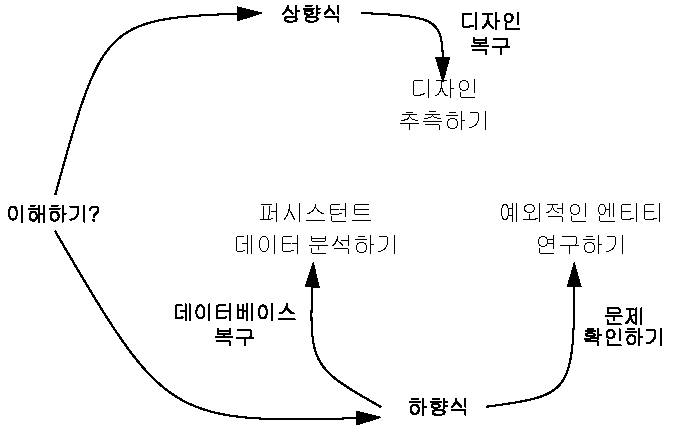
\includegraphics[width=\textwidth]{oldInitialUnderstandingMap.pdf}
\caption{소프트웨어 시스템의 \charef{초기 이해}{InitialUnderstanding}를 구하고 이를 상위 수준의 표현으로 변환한다.}
\figlabel{InitialUnderstandingMap}
\end{center}
\end{figure}

이러한 각 패턴에 할애해야 하는 시간은 리엔지니어링 프로젝트의 목표에 따라 크게 달라진다. 원칙적으로 이러한 패턴 중 어느 것도 오래 걸리지 않지만 각 패턴은 여러 번 적용해야 한다. 팀이 나머지 프로젝트를 진행할 만큼 충분히 이해했는지 여부는 패턴을 적용한 후에야 평가할 수 있기 때문에 얼마나 많은 주기가 필요할지 예측할 수 없다. 따라서 이러한 패턴은 사례별로 적용해야 한다.

\subsection*{다음 단계}

여러분이 추가로 이해한 내용을 프로젝트 계획에 반영해야 한다. 예를 들어 \patref{퍼시스턴트 데이터 분석하기}{AnalyzeThePersistentData} 및 \patref{디자인에 대한 추측}{SpeculateAboutDesign}은 시스템의 일부를 문서화하며, 이 문서를 기회(Opportunity)로 사용해야 한다. 반면에 \patref{예외적인 엔티티 연구하기}{StudyTheExceptionalEntities}를 사용하면 의심스러운 컴포넌트를 발견할 수 있으며, 이러한 컴포넌트는 리스크(Risk)로 관리해야 한다.

여러분이 충분히 이해하여 충분한 기초를 마련했다면 나머지 프로젝트에 중요한 컴포넌트에 대한 세부 정보를 채워 넣어야 한다. \chapgref{디테일 모델 캡처}{DetailedModelCapture}에 설명된 활동이 이러한 세부 정보를 채우는 데 도움이 될 수 있다.

%=================================================================
%:PATTERN -- {Analyze the Persistent Data}
\pattern{퍼시스턴트 데이터 분석하기}{AnalyzeThePersistentData}

\intent{데이터베이스 시스템 내부에 보관해야 할 정도로 중요한 개체에 대해 학습한다.}

\subsection*{문제}

Which object structures represent the valuable data ?
어떤 개체 구조가 중요한 데이터를 나타낼까요?

\emph{이 문제는 다음과 같은 이유로 어렵다.}

\begin{bulletlist}
\item 귀중한 데이터는 외부 저장 장치(예: 파일 시스템, \ind{database})에 안전하게 보관해야 한다. 그러나 이러한 데이터 저장소는 종종 다락방(attic)\footnote{서양에서는 오래된 물건을 다락방에 보관하곤 한다. -옮긴이} 역할을 하므로 거의 정리되지 않고 많은 정크를 포함할 수 있다.

\item 메모리에 로드될 때 중요한 데이터는 복잡한 객체 구조로 표현된다. 안타깝게도 외부 저장 장치에서 제공하는 데이터 구조와 주 메모리에 있는 객체 구조 사이에는 큰 차이가 있다. 예를 들어 상속 관계는 레거시 데이터베이스에서 명시적으로 제공되는 경우가 거의 없다.

\item ``값(Valuable)''은 상대적인 속성이다. 저장된 데이터의 상당 부분이 리엔지니어링 프로젝트와 관련이 없을 수 있다.
\end{bulletlist}

\emph{그러나 이 문제를 해결할 수 있는 이유는 다음과 같다.}

\begin{bulletlist}
\item 소프트웨어 시스템은 데이터를 영구적으로 유지하기 위해 어떤 형태의 데이터베이스를 사용합한. 따라서 데이터베이스 내부의 데이터에 대한 정적 설명을 제공하는 일종의 데이터베이스 스키마가 존재한다.

\item 데이터베이스에는 데이터베이스 내부의 실제 개체를 검사하는 데 필요한 도구가 함께 제공되므로 레거시 데이터의 존재를 활용하여 결과를 미세 조정할 수 있다.

\index{데이터베이스!스키마}
\item 구현 언어의 데이터 구조를 데이터베이스 스키마에 매핑하는 데 어느 정도 전문 지식이 있으며, 데이터베이스 스키마에서 클래스 다이어그램을 재구성할 수 있을 정도이다.

\item 시스템의 기능과 프로젝트의 목표를 대략적으로 이해하고 있으므로(예: \charef{첫 번째 접근}{FirstContact}를 통해 얻은 정보) 데이터베이스의 어느 부분이 프로젝트에 유용한지 평가할 수 있다.
\end{bulletlist}

\subsection*{해결}

데이터베이스 스키마를 분석하여 어떤 구조가 가치 있는 데이터를 나타내는지 필터링한다. 나머지 팀원들을 위해 해당 지식을 문서화할 수 있도록 해당 엔티티를 나타내는 \subind{UML}{클래스 다이어그램}을 도출한다.

\subsubsection*{단계}

아래 단계에서는 시스템이 객체 지향 애플리케이션의 일반적인 경우인 \emph{관계형 데이터베이스(relational database)}를 사용한다고 가정한다. 그러나 다른 종류의 데이터베이스 시스템을 사용하는 경우에도 이러한 단계 중 많은 부분이 여전히 적용될 수 있다. 단계 자체는 가이드라인일 뿐이므로 직관과 역추적을 충분히 활용하여 반복적으로 적용해야 한다.

\noindent
\emph{준비.}
관계형 데이터베이스 스키마에서 클래스 다이어그램을 도출하려면 먼저 테이블을 클래스로 표현하는 초기 모델을 준비한다. 소프트웨어 도구를 사용하여 이 작업을 수행할 수도 있지만 인덱스 카드 세트를 사용하는 것도 좋다.

\begin{enumerate}
  \item 모든 테이블 이름을 열거하고 각 테이블에 대해 같은 이름의 클래스를 만든다.

  \item 각 테이블에 대해 모든 열 이름을 수집하고 이를 해당 클래스에 속성으로 추가한다.

  \item 각 테이블에 대해 후보 키(candidate key)를 결정한다. 그중 일부는 데이터베이스 스키마에서 직접 읽을 수 있지만 일반적으로 더 자세한 분석이 필요하다. 후보 키를 제안하는 경우가 많으므로 모든 (고유) 인덱스를 반드시 확인하자. 명명 규칙(ID 또는 \#을 포함한 이름)도 후보 키를 나타낼 수 있다. 의심스러운 경우 데이터 샘플을 수집하여 후보 키가 데이터베이스 모집단 내에서 실제로 고유한지 확인한다.

  \item 테이블 간의 모든 외래 키(foreign key) 관계를 수집하고 해당 클래스 간의 연결을 생성한다. 외래 키 관계는 데이터베이스 스키마에 명시적으로 유지되지 않을 수 있으므로 열 유형과 명명 규칙(naming convention)을 통해 이를 유추해야 한다. 여기에는 동음이의어(homonym)(=열 이름과 유형은 동일하지만 의미는 다른)와 동의어(synonym)(=열 이름이나 유형은 다르지만 의미는 동일한)가 존재할 수 있으므로 신중한 분석이 필요하다. 이러한 어려움에 대처하려면 최소한 인덱스와 뷰 선언이 빈번한 탐색 경로를 가리키므로 이를 확인해야 한다. 가능하면 데이터베이스에 대해 실행되는 \ind{SQL} 문의 조인 절(join clause)을 확인한다. 마지막으로, 데이터 샘플을 검사하여 특정 외래 키 관계를 확인(verify)하거나 반박(refute)한다.

\end{enumerate}

\begin{figure}
\begin{center}
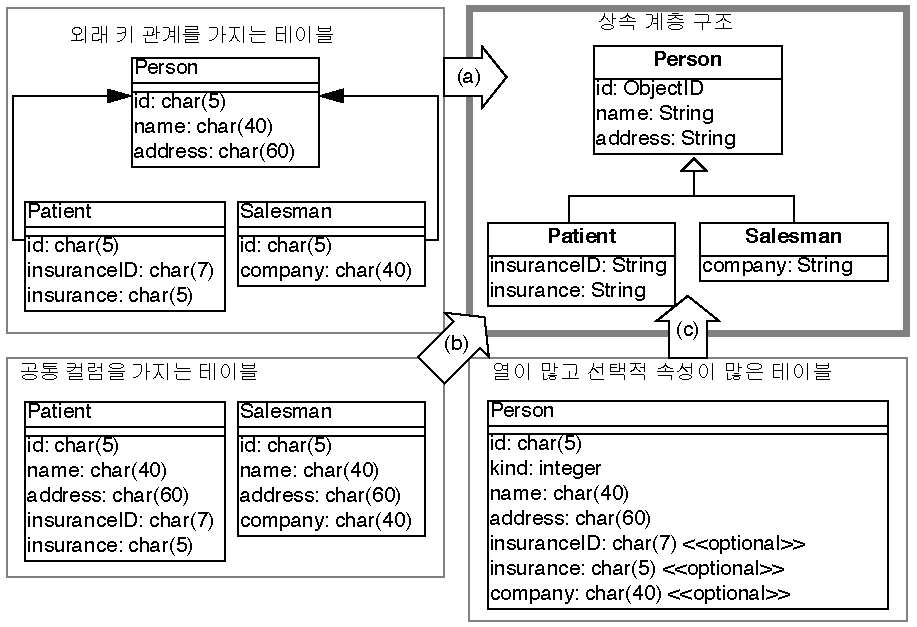
\includegraphics[width=\textwidth]{InitialMappingRelations}
\caption{계열 관계형 테이블을 상속 계층 구조에 매핑하기. (a) 일대일, (b) 롤다운, (c) 롤업}
\figlabel{InitialMappingRelations}
\end{center}
\end{figure}

\noindent
\emph{상속 통합(Incorporate inheritance).}
위의 단계를 마치면 관계형 데이터베이스에 저장되는 테이블을 나타내는 클래스 집합을 갖게 된다. 그러나 관계형 데이터베이스는 상속 관계를 나타낼 수 없기 때문에 외래 키에서 상속 관계를 유추해야 한다. (5-7단계에서 상속 관계의 세 가지 표현에 대한 용어는 \cite{Fros94a}에서 유래했다.)

\begin{enumerate}\setcounter{enumi}{4}
  \item \emph{일대일(One to one)} (\figref{InitialMappingRelations} (a)). 기본 키가 다른 테이블의 외래 키 역할도 하는 테이블을 확인한다. 이러한 외래 키는 상속 관계를 나타낼 수 있기 때문이다. 이러한 테이블에 대해 실행되는 SELECT 문을 검사하여 일반적으로 이 외래 키에 대한 조인을 포함하는지 확인한다. 이 경우 테이블 이름과 해당 소스 코드를 분석하여 이 외래 키가 실제로 상속 관계를 나타내는지 확인한다. 그렇다면 외래 키에 해당하는 연결을 상속 관계로 변환한다.

  \item \emph{롤다운(Rolled down)} (\figref{InitialMappingRelations} (b)). 클래스 계층 구조가 여러 테이블에 분산되어 있고 각 테이블이 하나의 비추상 클래스를 나타내는 상황을 나타낼 수 있으므로 열 정의의 공통 집합이 있는 테이블을 확인한다. 중복된 열 정의의 각 클러스터에 대해 공통 수퍼클래스를 정의하고 해당 속성을 새 클래스 내부로 이동한다. 소스 코드에서 새로 생성된 클래스에 적용할 수 있는 이름을 확인한다.

  \item \emph{롤업(Rolled up)} (\figref{InitialMappingRelations} (c)). 열이 많고 선택적 속성이 많은 테이블은 전체 클래스 계층 구조가 단일 테이블에 표시되는 상황을 나타낼 수 있으므로 확인한다. 이러한 테이블을 발견한 경우 이 테이블에 대해 실행되는 모든 SELECT 문을 검토한다. 이러한 SELECT 문이 명시적으로 열의 하위 집합을 요청하는 경우 요청된 하위 집합에 따라 이 하나의 클래스를 여러 클래스로 나눌 수 있다. 이러한 클래스의 이름에 대해 열거형 유형 번호를 포함하는 'kind' 열과 같은 하위 유형 정보의 인코딩이 있는지 확인한다.

\end{enumerate}

\noindent
\emph{연관 통합(Incorporate associations).}
데이터베이스에서 추출한 클래스 다이어그램이 너무 작을 수 있다. 실제 상속 계층 구조의 클래스가 새로운 속성을 정의하지 않아 데이터베이스에서 누락되었을 수 있다. 또한 테이블 및 열 이름이 이상하게 들릴 수도 있다. 따라서 클래스 다이어그램을 소스 코드와 비교하여 확인하면 추가적인 인사이트를 얻을 수 있으므로(\patref{디자인 추측하기}{SpeculateAboutDesign} 참조), 이를 고려해 보자. 그런 다음 나머지 연관성을 구체화한다.

\begin{enumerate}\setcounter{enumi}{7}
  \item 연관 클래스(association class), 즉 두 개체가 연관되어 있다는 사실을 나타내는 클래스를 결정한다. 가장 일반적인 예는 두 개의 외래 키로 구성된 후보 키를 가진 테이블로 표현되는 다대다 연결이다. 일반적으로 후보 키가 여러 외래 키의 연결인 모든 테이블은 연결 클래스의 잠재적 사례이다.

  \item 상호 보완적인 연관성(complementary association)을 병합한다. 클래스 A가 클래스 B에 대한 외래 키 연관을 갖고 있고 클래스 B가 클래스 A에 대한 역외래 키를 갖는 경우가 있다. 이 경우 두 연관을 양방향으로 탐색 가능한 단일 연관으로 병합한다.

  \item \ind{외래 키}(foreign key) 대상을 해결한다. 데이터베이스에서 상속 계층이 롤업 또는 롤다운된 경우 테이블을 구성하는 클래스에서 테이블이 분해된 후 외래 키 대상이 모호해질 수 있다. 외래 키 대상이 계층 구조에서 너무 높거나 낮을 수 있으며, 이 경우 해당 연결에 참여하는 클래스가 너무 적거나 너무 많을 수 있다. 이러한 상황을 해결하려면 일반적으로 데이터 샘플과 \ind{SQL} 문을 분석하여 실제로 어떤 클래스가 연결에 참여하는지 확인해야 한다.

  \item 한정된 연관(qualified association), 즉 특정 조회 키(look-up key) 혹은 한정자(qualifier))를 제공하여 탐색할 수 있는 연관을 식별한다. 일반적인 예는 주문 번호가 한정자 역할을 하는 일대다 연결이다. 일반적으로 후보 키가 외래 키와 추가 열을 결합하는 모든 테이블은 잠재적인 한정자 연결이며, 추가 열은 한정자를 나타낸다.

  \item 연관(association)에 대한 다중성(multiplicity)을 기록한다. 모든 연관은 외래 키 관계에서 파생되므로 모든 연결은 구조상 선택적 1 대 다 연관이다. 그러나 null이 아닌 선언, 인덱스 및 데이터 샘플을 검사하여 연관의 각 역할에 대한 최소 및 최대 다중성을 결정할 수 있는 경우가 많다.

\end{enumerate}

\noindent
\emph{검증.}
데이터베이스 스키마만으로는 완전한 클래스 다이어그램을 도출하기에는 근거가 너무 약하다는 반복되는 지적에 유의하자. 다행히도 레거시 시스템에는 채워진 데이터베이스와 그 데이터베이스를 조작하는 프로그램이 있다. 따라서 데이터 샘플과 내장된 \ind{SQL} 문을 사용하여 재구성된 클래스를 검증할 수 있다.

\begin{bulletlist}
\item \emph{데이터 샘플.}
데이터베이스 스키마는 기본 데이터베이스 시스템과 모델에서 허용하는 제약 조건만 지정한다. 그러나 문제 도메인에는 스키마에 표현되지 않은 다른 제약 조건이 포함될 수 있다. 데이터베이스에 저장된 실제 데이터의 샘플을 검사하여 다른 제약 조건을 유추할 수 있다.

\item \emph{\ind{SQL} 문(\ind{SQL} statements).}
관계형 데이터베이스 스키마의 테이블은 외래 키를 통해 연결된다. 그러나 명시적인 외래 키가 없더라도 일부 테이블은 항상 함께 액세스되는 경우가 있다. 따라서 데이터베이스 엔진에 대해 실제로 어떤 쿼리가 실행되는지 확인하는 것이 좋다. 이를 수행하는 한 가지 방법은 프로그램에 포함된 모든 \ind{SQL} 문을 추출하는 것이다. 또 다른 방법은 데이터베이스 시스템과 함께 제공되는 추적 기능을 통해 실행된 모든 쿼리를 분석하는 것이다.

\end{bulletlist}

\noindent
\emph{오퍼레이션 통합(Incorporate operations).}
데이터베이스에서 추출한 \subind{UML}{클래스 다이어그램}은 데이터 구조만 나타내며, 그 구조를 조작하는 데 사용된 오페레이션은 나타내지 않는다는 점을 분명히 알아야 한다. 따라서 결과 클래스 다이어그램은 반드시 불완전할 수밖에 없다. 코드를 데이터베이스에서 추출한 모델과 비교하면(\patref{디자인 추측하기}{SpeculateAboutDesign} 및 \patpgref{계약 찾기}{LookForTheContracts} 참조) 추출된 클래스에 대한 연산을 통합할 수 있다.

\subsection*{트레이드오프}

\subsubsection*{장점}

\begin{bulletlist}
\item \emph{팀 커뮤니케이션을 개선한다.} 데이터베이스 스키마를 캡처하면 리엔지니어링 팀 내 및 프로젝트와 관련된 다른 개발자(특히 유지보수 팀)와의 커뮤니케이션이 개선된다. 또한 많은 개발 방법론에서 데이터베이스 설계의 중요성을 강조하기 때문에 프로젝트와 관련된 모든 사람은 아니더라도 많은 사람들이 데이터 스키마가 있다는 사실에 안심할 수 있다.

\item \emph{가치 있는 데이터에 집중하자.} 데이터베이스는 백업과 보안을 위한 특별한 기능을 제공하므로 중요한 데이터를 저장하기에 이상적인 장소이다. 데이터베이스 스키마를 이해하면 중요한 데이터를 추출하여 향후 리엔지니어링 활동 중에 보존할 수 있다.
\end{bulletlist}

\subsubsection*{단점}

\begin{bulletlist}
\item \emph{범위가 제한된다.}
데이터베이스는 오늘날 많은 소프트웨어 시스템에서 매우 중요하지만 전체 시스템에서 차지하는 비중은 극히 일부에 불과하다. 따라서 이 패턴에만 의존하여 시스템을 전체적으로 파악할 수는 없다.

\item \emph{정크 데이터가 포함되어 있다.}
데이터베이스에는 가치 있는 데이터보다 훨씬 더 많은 데이터가 포함되며, 레거시 시스템이 얼마나 오래되었는지에 따라 아무도 제거하지 않아서 많은 정크 데이터가 저장되어 있을 수 있다. \emph{따라서 복구한 데이터베이스 스키마를 리엔지니어링 프로젝트의 요구 사항과 일치시켜야 한다.}

\item \emph{데이터베이스 전문 지식이 필요하다.}
이 패턴을 사용하려면 기본 데이터베이스에 대한 많은 지식과 데이터베이스 스키마를 구현 언어에 매핑하는 구조가 필요하다. 따라서 이 패턴은 선택한 데이터베이스에서 구현 언어로의 매핑에 대한 전문 지식을 갖춘 사람이 적용하는 것이 바람직하다.

\item \emph{시스템의 동작 내용이 부족하다(Lacks behavior).}
데이터베이스에서 추출한 클래스 다이어그램은 매우 데이터 지향적이며 동작이 거의 또는 전혀 포함되어 있지 않다. 진정한 객체 지향 클래스 다이어그램은 데이터와 동작을 모두 캡슐화해야 하므로 그런 의미에서 데이터베이스 스키마는 그림의 절반만 보여준다. 그러나 일단 데이터베이스 모델이 존재하면 나중에 누락된 동작을 추가할 수 있다.
\end{bulletlist}

\subsubsection*{어려움}

\begin{bulletlist}
\item \emph{오염된 데이터베이스 스키마.}
데이터베이스 스키마 자체가 항상 중요한 객체에 대한 클래스 다이어그램을 재구성하는 데 가장 좋은 정보 소스는 아니다. 많은 프로젝트에서 데이터베이스 액세스를 최적화해야 하므로 데이터베이스 스키마를 깨끗하게 유지하는 것을 희생하는 경우가 많다. 또한 데이터베이스 스키마 자체는 시간이 지남에 따라 진화하기 때문에 서서히 성능이 저하된다. \emph{따라서 데이터 샘플과 내장된 \ind{SQL} 문을 분석하여 클래스 다이어그램을 개선하는 것이 매우 중요하다.}
\end{bulletlist}

\subsection*{예시}

\emph{XDoctor}를 인수하면서 여러분의 회사는 기존 고객층을 계속 지원하기로 약속했다. 특히 고객에게 단 1바이트의 데이터도 손실되지 않을 것이라고 보장했는데, 이제 상사가 데이터베이스 구조를 복구해 달라고 요청한다. 자신의 제품 사용 경험을 통해 의사들이 환자 파일에 많은 관심을 갖고 있으며 그러한 정보를 잃어버리는 것은 용납할 수 없다는 것을 알고 있다. 따라서 데이터베이스 내부에 환자 파일이 저장되는 방식을 분석하는 것부터 시작하기로 결정한다.

\begin{figure}
\begin{center}
\includegraphics[width=\textwidth]{InitialQualified}
\caption{외래 키(patientID)와 두 개의 추가 열(date, nr)로 구성된 키를 통해 한정된 연관(qualified association)을 식별한다.}
\figlabel{InitialQualified}
\end{center}
\end{figure}

먼저 모든 테이블 이름을 검색하여 \lct{Patient}라는 이름의 테이블을 찾으려고 하지만 안타깝게도 찾을 수 없다. 그러나 \lct{Person}이라는 테이블에서 거의 일치하는 항목이 있는데, \lct{insuranceID}와 같은 열 이름을 보면 적어도 일부 환자 정보가 저장되어 있음을 알 수 있다. 그럼에도 불구하고 많은 열 이름이 선택 사항이므로 환자 정보가 다른 종류의 정보와 혼합된 롤업된 표현이 의심된다. 따라서 소스 코드를 확인하고 \lct{Person} 테이블을 쿼리하는 모든 내장된 SQL 문을 찾습는다(예: \lct{grep "SELECT * Person"}). 실제로 이러한 쿼리가 사용되는 두 개의 클래스, 즉 \lct{Patient}와 \lct{Salesman}이 있으며 각 클래스에서 쿼리된 열의 하위 집합에서 \figref{InitialMappingRelations}에 표시된 상속 계층을 유추할 수 있다.

이제 \lct{Patient}를 복구했으므로 환자가 받은 치료를 저장하는 테이블을 찾기 시작한다. 실제로 \lct{Person} 테이블에 대한 외래 키가 있는 \lct{Treatment} 테이블이 있다. 그러나 \lct{Person}을 \lct{Patient} 및 \lct{Salesman} 클래스로 분해했으므로 외래 키의 대상을 확인해야 한다. \lct{patientID}를 통해 \lct{Person} 및 \lct{Treatment} 테이블을 조인하면(SELECT DISTINCT name, kind FROM Person, Treatment WHERE Person.id = Treatment.patientID) 선택한 모든 사람이 실제로 \lct{Patient}에 해당하는 종류를 가지고 있음을 확인할 수 있다. 따라서 외래 키의 대상을 \lct{Treatment}에서 \lct{Patient}로 설정한다(\figref{InitialMappingRelations}의 왼쪽 참조). 다음으로 \lct{Treatment}에 정의된 인덱스를 확인하고 \lct{patientID - date - nr} 열에 고유 인덱스가 있음을 확인하여 이 열이 후보 키 역할을 한다는 결론을 내린다. lct{Treatment}의 후보 키는 두 개의 추가 열과 결합된 외래 키로 구성되어 있으므로 한정된 연관(qualified association)이 의심된다. 이 가정을 확인하기 위해 데이터 샘플(\lct{SELECT name, date, nr FROM Person, Treatment WHERE Person.id = Treatment.patientID ORDER BY name, date, nr})을 분석하여 날짜와 번호가 특정 환자의 치료를 고유하게 식별하는지 확인한다. 결과적으로 외래 키를 각 역할에 대해 다중성 1(multiplicity of one)을 가지는 정규화된 연관 had-treatment로 변환한다.

\subsection*{근거}

\index{블라하, 마이클}
\begin{quotation}
\noindent
\emph{객체 모델은 데이터 구조를 간결하게 설명하고 구조적 제약사항을 포착하기 때문에 데이터베이스 애플리케이션에 중요하다. }

\hfill --- 마이클 블라하 외  \cite{Blah98a} 
\end{quotation}

잘 정의된 중앙 데이터베이스 스키마를 갖는 것은 영구 데이터를 다루는 대규모 소프트웨어 프로젝트에서 흔히 볼 수 있는 관행이다. 특정 데이터 구조에 액세스하는 방법에 대한 공통 규칙을 지정할 뿐만 아니라 팀원 간에 작업을 분담하는 데도 큰 도움이 된다. 따라서 다른 리버스 엔지니어링 활동을 진행하기 전에 데이터베이스의 정확한 모델을 추출하는 것이 좋다.

데이터베이스 모델을 추출하는 것은 본질적으로 상향식(bottom-up) 접근 방식이다. 데이터베이스 스키마에 포함된 대략적인 정보에서 시작하여 만족스러운 클래스 다이어그램이 나올 때까지 다듬는 것이다. 데이터베이스 스키마는 이미 더 자세한 표현에서 추상화된 것이기 때문에 이러한 상황에서는 상향식 접근 방식이 매우 효과적이다.

\index{리엘, 아서}
\begin{quotation}
\noindent
\emph{모든 데이터는 해당 클래스 내에서 숨겨야 한다.}

\hfill --- 아서 리엘, 휴리스틱 2.1 \cite{Riel96a}
\end{quotation}

정보 숨김은 중요한 설계 원칙이며, 대부분의 저자는 클래스의 경우 모든 데이터가 클래스 내에서 캡슐화되고 해당 클래스에 정의된 연산을 통해서만 액세스해야 한다는 데 동의한다. 안타깝게도 데이터베이스에서 추출한 클래스 다이어그램은 데이터베이스의 특성 때문에 모든 데이터를 노출하게 된다. 따라서 이 클래스 다이어그램은 데이터베이스에 대한 잘 설계된 인터페이스를 향한 첫 단계일 뿐이다.

\subsection*{알려진 용도}

데이터베이스 시스템의 리버스 엔지니어링 및 리엔지니어링은 잘 탐구된 연구 분야이다 \cite{Arno92a} \cite{Mull00a}. 여러 실험에 따르면 잘못 설계된 데이터베이스 시스템에서도 데이터베이스 구조를 복구하는 것이 가능하다는 사실이 밝혀졌다. 예를 들어, 주요 RDBMS 공급업체의 데이터 사전과 기계 부품에 대한 데이터를 저장하는 운영 데이터베이스의 리버스 엔지니어링에 관한 실험에 관한 보고서 \cite{Prem94a}를 참조하자. \cite{Hain96a}는 프로토타입 데이터베이스 리버스 엔지니어링 툴킷과 이 툴킷이 적용된 5가지 산업 사례에 대해 설명한다. 데이터베이스 리버스 엔지니어링의 예측 불가능한 특성을 설명하기 위해 \cite{Jahn97b}에서는 관계형 데이터베이스 스키마에서 클래스 다이어그램을 추출하는 도구의 핵심으로 퍼지 추론 엔진을 사용하는 것에 대해 설명한다.

\subsection*{다음 단계}

\patref{퍼시스턴트 데이터 분석하기}{AnalyzeThePersistentData}은 소프트웨어 시스템의 영구 데이터에 대한 클래스 다이어그램을 생성한다. 이러한 클래스 다이어그램은 매우 대략적이며 주로 데이터의 구조에 관한 것이지 데이터의 동작에 관한 것이 아니다. 그러나 \patref{디자인 추측하기}{SpeculateAboutDesign} 및 \patpgref{계약 찾기}{LookForTheContracts}를 적용하여 더 구체화할 수 있는 이상적인 초기 가설로 사용될 수 있다.

다른 데이터베이스로 마이그레이션해야 하는 경우, 데이터베이스 모델에 대한 이해를 \chapgref{테스트라는 생명 보험}{TestsYourLifeInsurance}에 설명된 대로 테스트 스위트에 적용(cast)해야 합니다.

관계형 데이터베이스에 객체 지향 데이터 구조를 매핑하는 다양한 방법을 설명하는 패턴, 관용구 및 패턴 언어가 존재한다는 점에 유의하자 \cite{Brow96d}. \cite{Kell98a}. 데이터베이스 스키마를 리버스 엔지니어링할 때 이를 참조하면 도움이 될 수 있다.

%=================================================================
%:PATTERN -- {Speculate about Design}
\pattern{디자인 추측하기}{SpeculateAboutDesign}

\intent{소스코드에 대한 디자인의 가설을 확인하여 소스코드에 대한 디자인을 점진적으로 구체화(refine)한다.}

\subsection*{문제}

소스 코드에서 디자인 개념이 표현되는 방식을 어떻게 복구할 수 있는가?

\emph{이 문제는 다음과 같은 이유로 어렵다.}

\begin{bulletlist}

\item 많은 디자인 개념이 있으며 사용되는 프로그래밍 언어에서 이를 표현하는 방법은 무수히 많다.

\item 소스 코드의 대부분은 디자인과 관련이 없으며 오히려 다음과 같은 문제와 관련이 있다. 구현 문제(글루 코드, 사용자 인터페이스 제어, 데이터베이스 연결 등)와 관련이 있다.
\end{bulletlist}

\emph{그러나 이 문제를 해결할 수 있는 이유는 다음과 같다.}

\begin{bulletlist}
\item 시스템 기능에 대한 \emph{대략적인 이해를 통해}(예를 들어 를 통해 얻은 \patpgref{문서 스키밍하기}{SkimTheDocumentation} 및 \patpgref{데모 중 인터뷰하기}{InterviewDuringDemo}를 통해 얻을 수 있음), 따라서 초기 어떤 디자인 문제를 해결해야 하는지 알 수 있다.

\item \emph{개발 전문 지식(development expertise)}이 있으므로 해당 문제를 어떻게 디자인할지 상상할 수 있다. 문제를 어떻게 설계할지 상상할 수 있다.

\item 소스 코드의 주요 구조에 대해 \emph{어느 정도 익숙하다}(예를 들어 \patpgref{한 시간 안에 모든 코드 읽기}{ReadAllTheCodeInOneHour}로 얻은 정보가 있다). 그러므로 길을 찾을 수 있다.
\end{bulletlist}

\subsection*{해결}

개발 전문 지식을 활용하여 디자인을 나타내는 가상의 클래스 다이어그램을 만들어보자. 클래스 다이어그램의 이름이 소스 코드에 있는지 확인하고 그에 따라 모델을 조정하여 해당 모델을 구체화하자. 클래스 다이어그램이 안정화될 때까지 이 과정을 반복하자.

\subsubsection*{단계}
\begin{enumerate}
  \item 시스템에 대한 이해를 바탕으로 소스 코드에서 무엇을 기대할 수 있는지에 대한 초기 가설 역할을 하는 클래스 다이어그램을 작성하자. 클래스, 연산 및 속성의 이름은 자신의 경험과 잠재적인 명명 규칙을 바탕으로 추측하자(\patpgref{문서 스키밍하기}{SkimTheDocumentation} 참조).

  \item 클래스 다이어그램에 있는 이름(즉, 클래스, 속성 및 연산 이름)을 열거하고 사용 가능한 도구를 사용하여 소스 코드에서 해당 이름을 찾아보자. 소스 코드 내의 이름이 항상 그 이름이 나타내는 개념과 일치하는 것은 아니므로 주의하자.\footnote{리버스 엔지니어링 경험 중 하나에서 영어와 독일어가 혼용된 소스 코드를 마주한 적이 있었다. 예상할 수 있듯이 이것은 문제를 매우 복잡하게 만든다.} 이를 방지하기 위해 소스 코드에 나타날 가능성에 따라 이름의 순위를 매길 수 있다.

  \item 소스 코드에 나타나는 이름을 추적하고(가설 확인) 소스 코드의 식별자와 일치하지 않는 이름을 추적하자(가설과 모순됨). 불일치는 시스템을 이해할 때 반드시 거쳐야 하는 학습 과정을 촉발하므로 긍정적이라는 점을 기억하자.

  \item 불일치를 기반으로 클래스 다이어그램을 조정한다. 이러한 조정에는 다음이 포함될 수 있다.

(a) \emph{이름 바꾸기(renaming)}: 소스 코드에서 선택한 이름이 가설과 일치하지 않는 것을 발견한 경우 사용한다.

(b) \emph{리모델링(remodelling)}:디자인 개념의 소스 코드 표현이 모델에 있는 것과 일치하지 않는다는 것을 알게 될 때 사용한다. 예를 들어 연산을 클래스로 변환하거나 속성을 연산으로 변환할 수 있다.

(c) \emph{확장(extending)}: 클래스 다이어그램에 나타나지 않는 소스 코드의 중요한 요소를 발견한 경우 사용한다.

(d) \emph{대안 찾기(seeking alternatives)}: 소스 코드에서 디자인 개념을 찾을 수 없는 경우 사용한다. 여기에는 불일치가 거의 없는 경우 동의어를 시도하는 것이 포함될 수 있지만 다음과 같은 경우도 수반될 수 있다. 불일치가 많을 때는 완전히 다른 클래스 다이어그램을 정의해야 할 수도 있다.

  \item 만족스러운 클래스 다이어그램을 얻을 때까지 2~4단계를 반복한다.

\end{enumerate}

\subsubsection*{변형}

\variant{비즈니스 객체에 대해 추측한다.}
시스템 설계에서 중요한 부분은 문제 도메인(problem domain)의 개념이 소스 코드에서 클래스로 표현되는 방식이다. 이 패턴의 변형을 사용하여 소위 ``비즈니스 객체''를 추출할 수 있다.

초기 가설을 구축하는 한 가지 방법은 요구 사항의 명사 구문을 초기 클래스 이름으로, 동사 구문을 초기 메서드 이름으로 사용하는 것이다(\cite{Wirf90b} \cite{Bell97a} \cite{Booc94a}에서 클래스와 그 책임(responsability) 찾기에 대해 자세히 다루고 있다). 어떤 객체가 어떤 역할을 수행하는지 알아내는 데 도움이 될 수 있는 사용 시나리오를 통해 이 정보를 보강해야 할 수도 있다. \patpgref{데모 중 인터뷰하기}{InterviewDuringDemo}를 통해서 이러한 시니리오를 구할 수 있을 것이다. (참조 시나리오 및 사용 사례는 \cite{Jaco92a} \cite{Schn98a}, 역할 모델링에 대해서는 \cite{Reen96a} \cite{Rieh98a}를 참조하자.)

\variant{패턴에 대해 추측한다.}
패턴은 ``주어진 맥락에서 공통적인 디자인 문제에 대한 반복적인 해결책''이다. 특정 패턴이 어디에 적용되었는지 알면 기본 시스템 설계에 대해 많은 것을 알 수 있다. 이 변형은 아키텍처 \cite{Busc96a}, 분석 \cite{Fowl97b} 또는 디자인 패턴 \cite{Gamm95a}의 발생에 대한 가설을 검증한다.

\variant{아키텍처에 대해 추측한다.}
``소프트웨어 \ind{아키텍처}는 소프트웨어 시스템의 하위 시스템과 컴포넌트 및 이들 간의 관계에 대한 설명이다.'' \cite{Busc96a}(일명 컴포넌트와 커넥터(Components and Connectors) \cite{Shaw96a}). 소프트웨어 아키텍처는 일반적으로 시스템의 대략적인 수준 설계와 연관되어 있으므로 전체 구조를 이해하는 데 매우 중요합니다. 소프트웨어 아키텍처는 리버스 엔지니어링이 매우 어려운 영역인 여러 협력 프로세스가 있는 분산 시스템의 맥락에서 특히 관련이 있다.

이 변형은 어떤 컴포넌트와 커넥터가 존재하는지, 또는 분산 시스템의 맥락에서 어떤 프로세스가 존재하는지, 어떻게 시작되고 어떻게 종료되며 어떻게 상호 작용하는지에 대한 가설을 세우고 구체화한다. 아키텍처 패턴의 카탈로그는 \cite{Busc96a}를, 잘 알려진 아키텍처 스타일 목록은 \cite{Shaw96a}를 참조하자. 동시 프로그래밍에 적용될 수 있는 몇 가지 일반적인 패턴과 이디엄는 \cite{Lea96a}를, 분산 시스템의 아키텍처 패턴은 \cite{Schm00a}를 참조하자.

\subsection*{트레이드오프}

\subsubsection*{장점}

\begin{bulletlist}
\item \emph{규모확장이 잘 지원된다.}
소스 코드에서 무엇을 찾을 수 있을지 추측하는 것은 규모 확장에 유리한 기법이다. 이는 대규모 객체 지향 프로그램(100개 이상의 클래스)의 경우 상향식 접근 방식이 금방 비실용적이 되기 때문에 특히 중요하다.

\item \emph{투자는 성과를 돌려준다.}
이 기술은 리소스와 도구 측면에서 상당히 저렴하며, 이해의 양을 고려할 때 확실히 비용이 낮다.
\end{bulletlist}

\subsubsection*{단점}

\begin{bulletlist}
\item \emph{전문 지식이 필요하다.}
소스 코드에서 보이는 것을 인식하려면 이디엄, 패턴, 알고리즘, 기술에 대한 방대한 지식 레퍼토리가 필요하다. 따라서 이 패턴은 전문가가 적용하는 것이 바람직하다.

\item \emph{시간이 많이 소요된다.}
이 기술은 리소스와 도구 측면에서 상당히 저렴하지만 만족스러운 표현을 도출하기까지 상당한 시간이 필요하다.
\end{bulletlist}

\subsubsection*{어려움}

\begin{bulletlist}
\item \emph{일관성 유지는 어렵다.}
리버스 엔지니어링 프로젝트가 진행되고 소프트웨어 시스템에 대한 이해도가 높아지는 동안 클래스 다이어그램을 최신 상태로 유지할 계획을 세워야 한다. 그렇지 않으면 노력이 헛수고가 될 수 있다. 따라서 클래스 다이어그램이 소스 코드에 사용된 명명 규칙에 크게 의존하고 있는지, 클래스 다이어그램이 구성 관리 시스템의 제어를 받는지 확인하자.
\end{bulletlist}

\subsection*{예시}

\emph{XDoctor}를 인수하면서 여러분의 회사는 기존 고객층을 계속 지원하겠다고 약속했다. 그리고 스위스가 6개월 이내에 유로 지역에 가입할 예정이므로 마케팅 부서에서는 유로 전환이 제대로 지원되는지 확인하고자 한다. 1차 평가 결과 유로화가 어느 정도 지원되는 것으로 확인되었다(즉, 사용자 설명서에 설명되어 있고 \lct{Currency}라는 클래스가 존재한다). 이제 상사가 법적 의무를 충족할 수 있는지, 그렇지 않다면 소프트웨어를 조정하는 데 얼마나 걸리는지 조사해 달라고 요청한다.

\begin{figure}
\begin{center}
{\small (a) 미결 질문의 참고 사항으로 삽입된 초기 가설}
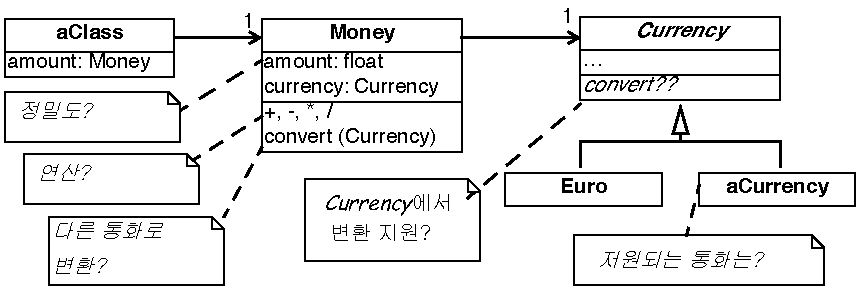
\includegraphics[width=\textwidth]{oldInitialCurrenciesA.pdf}
{\small (b) 소스 코드에 대한 검증을 거친 후 수정된 가설, 수정 사항은 참고 사항으로 표시}
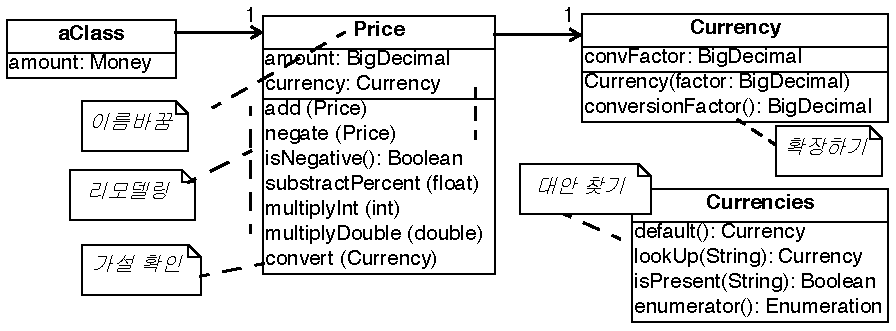
\includegraphics[width=\textwidth]{oldInitialCurrenciesB.pdf}
\caption{유로화 표시에 관한 가설 구체화하기. (a) 다양한 통화에 대한 서브클래스, (b) 통화에 대한 경량 패턴 접근 방식}
\figlabel{InitialCurrencies}
\end{center}
\end{figure}

이전 코드 검토에서 디자인이 상당히 훌륭하다는 것을 알았으므로 디자이너가 \patpgref{수량}{Quantity} 패턴을 일부 변형한 것을 적용했을 것으로 생각한다. 따라서 \figref{InitialCurrencies} (a)에 표시된 클래스 다이어그램의 형태로 초기 가설을 정의한다. 화폐의 양(부동 소수점 숫자)과 사용 중인 통화(\lct{Currency} 클래스의 인스턴스)의 두 가지 속성을 가진 \lct{Money} 클래스가 하나 있다. lct{Money} 클래스에서 더하기, 빼기, 곱하기, $\cdots$와 같은 표준 연산과 다른 통화로 변환하기 위한 연산 하나를 수행한다고 가정한다. \lct{Currency}에는 지원되는 모든 통화에 대한 서브클래스와 한 통화에서 다른 통화로의 변환을 지원하는 연산이 있어야 한다. 물론 몇 가지 질문에 대한 답이 없는 경우도 있으므로 클래스 다이어그램에 메모해 두어야 한다.

\begin{enumerate}
  \item \lct{Money}의 금액에 대한 정밀도는 어떻게 되는가?

  \item \lct{Money}의 인스턴스에서 어떤 연산이 허용되는가?

  \item \lct{Money}의 인스턴스를 다른 통화로 어떻게 변환하는가?

  \item 이 변환은 내부적으로 어떻게 이루어지는가? lct{Currency} 클래스의 지원은 어떻게 이루어지는가?

  \item 어떤 통화가 지원되나요?

\end{enumerate}

이러한 질문에 답하기 위해 소스 코드를 통해 가설을 검증하고 그에 따라 클래스 다이어그램을 조정한다. 파일 이름을 훑어보면 \lct{Currency} 클래스는 있지만 \lct{Money}라는 클래스는 없고, 모든 소스 코드를 grep 검색하면 \lct{Money} 클래스가 존재하지 않음을 확인할 수 있다. 어떤 패키지가 \lct{Currency}를 임포트하는지 검색하면 소스 코드의 실제 이름이 \lct{Price}라는 것을 금방 알 수 있고 그에 따라 \lct{Money} 클래스의 이름을 변경할 수 있다.

\lct{Price} 클래스 내부를 살펴보면 금액이 고정 소수점 숫자로 표시되어 있음을 알 수 있다. 아래와 같은 짧은 주석이 있다.

\begin{code}
Michael (Oct 1999) -- Bug Report #324 -- Replaced
Float by BigDecimal due to rounding errors in the
floating point representation. Trimmed down the
permitted calculation operations as well.
\end{code}

\lct{Price} 클래스의 인터페이스를 확인하면 계산 연산이 실제로 최소로 포함되어 있다는 것을 알 수 있다. 덧셈과 뺄셈(피연산자가 음수인 덧셈을 통해 뺄셈을 수행해야 함)과 백분율을 취하고 다른 숫자와 곱하기 위한 몇 가지 추가 연산만 있다. 그러나 가격 변환에 관한 가설을 확인하는 변환 연산도 볼 수 있다.

다음으로 \lct{Currency}의 서브클래스를 찾아보지만 아무것도 찾을 수 없을 것 같다. 당황한 여러분은 다른 해결책을 생각해 보기 시작하고 잠시 후 \patpgref{경량}{Flyweight} 패턴 적용의 가능성을 고려한다. 결국, 각 통화에 대해 별도의 서브클래스를 갖는 것은 추가 동작이 포함되지 않기 때문에 약간의 오버헤드가 발생한다. 또한 경량 패턴 접근 방식을 사용하면 단일 유로 객체로 유로 통화의 모든 발생을 표현함으로써 많은 메모리를 절약할 수 있다. 이 대안을 검증하려면 \lct{Currency}에 대한 생성자 메서드의 모든 발생을 찾아보면 \lct{grep Currency}가 트릭을 사용하여, 실제로 허용되는 모든 통화가 포함된 글로벌 테이블을 캡슐화하는 클래스를 발견하게 된다. 초기화 메서드를 살펴보면 다음과 같은 사실을 알 수 있다. 실제 테이블에는 두 가지 통화에 대한 항목이 포함되어 있다. 유로와 벨기에 프랑이다.

마지막으로, 실제 변환을 좀 더 자세히 살펴보기 위해 \lct{Price.convert} 연산과 \lct{Currency} 클래스의 내용을 살펴보자. 약간의 검색을 통해 각 \lct{Currency}에는 단일 변환 계수가 있다는 것을 알게 된다. 이렇게 하면 변환은 가능한 모든 통화 간에 두 가지 방식으로 작동해야 하지 않는가? 두 가지 방식으로 작동해야 하지 않을까? 하지만 conversionFactor 메서드의 모든 호출을 확인하면 변환이 기본 통화라는 개념을 중심으로 설계되었다는 것을 추론할 수 있다 (예: \lct{Currencies.default()} 연산). 그리고 \lct{conversionFactor}가 주어진 통화를 기본 통화로 변환한다. \lct{Price.convert 연산}을 확인하면 실제로 기본 통화에 대한 테스트가 있으며 이 경우 변환이 단순 곱셈에 해당한다는 것을 알 수 있다. 다른 경우에는 기본 통화로의 중간 변환을 포함하는 2단계 계산을 통해 변환이 수행된다.

결과가 상당히 만족스러우면 클래스 다이어그램을 그림 10(b)에 표시된 것과 같이 조정한다. 이 모델에는 원래 가설에 대한 수정 사항을 애너테이션(annotation)으로 표시되어 있으므로 동료들이 추론 과정을 재구성할 수 있도록 원래 모델과 수정된 모델을 모두 구성 관리 시스템에 저장한다. 또한 결과를 요약한 다음 보고서를 제출한다.

\noindent
\emph{유로로 변환.}
유로 변환 기능을 사용할 수 있지만 추가 작업이 필요하다. 하나의 중앙 클래스(Currencies)는 하나의 기본 통화(Currencies.default)를 포함하여 지원되는 통화 목록을 유지 관리한다. 유로로 변환하려면 이 클래스의 초기화를 변경하여 기본값이 유로가 되도록 해야 한다. 데이터베이스에 저장된 모든 가격도 변환해야 하지만 이는 우리가 연구한 범위를 벗어난다.

후속 작업을 수행합니다.

\begin{bulletlist}
\item 구성 파일에서 기본 통화 및 변환 계수를 읽도록 Currencies 클래스의 초기화를 조정한다.

\item \lct{Prices}을 어떻게 변환해야 하는지 데이터베이스를 확인한다.
\end{bulletlist}

\subsection*{근거}

\begin{figure}
\begin{center}
\includegraphics[width=\textwidth]{InitialWhiteNoise}
\caption{상향식 설계 추출 접근 방식으로 얻은 화이트 노이즈(white-noise). 이 그림은 중간 크기의 시스템에 대한 모든 메서드 호출과 속성의 접근으로 보강된 상속 계층 구조의 일부를 보여준다. 이 시각화는 \ind{CodeCrawler} \cite{Deme99c} \cite{Lanz99a}를 이용하였다.}
\figlabel{InitialWhiteNoise}
\end{center}
\end{figure}

디자인 추출에 대한 순진한 접근 방식은 상향식으로, 먼저 소스 코드에서 완전한 클래스 다이어그램을 만든 다음 노이즈를 제거하여 압축하는 것이다. 불행히도, 상향식 접근 방식은 대규모 시스템에서는 작동하지 않는다. 왜냐하면 일반적으로 많은 화이트 노이즈가 발생하기 때문이다(예를 들어 중간 규모의 시스템에 대한 연관성을 가진 상속 계층을 보여주는 \figref{InitialWhiteNoise}를 참조하자). 게다가 이러한 상향식 접근 방식은 중요한 개념 대신 관련 없는 노이즈에 집중하게 만들기 때문에 이해도를 크게 향상시키지 못한다.

\index{콕번, 앨리스터}
\begin{quotation}
\noindent
\emph{``우리는 일을 바로잡기 전에 일을 올바로 하지 못한다. We get things wrong before we get things right.''}

\hfill --- 앨리스터 콕번, \cite{Cock93a}
\end{quotation}

레거시 문제에 대한 진정한 이해를 얻으려면 학습 과정을 거쳐야 한다. \patref{디자인 추측하기}{SpeculateAboutDesign}는 이러한 학습 과정을 자극하기 위한 것이므로 가설과 모순되는 증거는 가설을 확인하는 증거만큼이나 가치가 있다. 실제로 불일치는 대안적인 해결책을 고려하고 장단점을 평가하게 하며, 바로 그 순간 진정한 이해가 생겨난다.

\subsection*{알려진 용도}

\cite{Murp97a}에는 Microsoft의 소프트웨어 엔지니어가 이 패턴(논문에서는 ``리플렉션 모델(Reflection Model)''이라고 함)을 적용하여 Microsoft Excel의 C 코드를 리버스 엔지니어링한 실험에 대한 보고서가 있다. 이 이야기의 좋은 점 중 하나는 그 소프트웨어 엔지니어가 시스템의 해당 부분을 처음 접한 사람이었고 동료들이 그에게 설명하는 데 많은 시간을 할애할 수 없었다는 것이다. 하지만 짧은 토론 끝에 그는 초기 가설을 세운 다음 소스 코드를 사용하여 점차적으로 이해를 구체화할 수 있었다. 이 논문에는 모델 지정, 모델에서 소스 코드로의 매핑, 모델에 대한 코드 확인에 도움이 되는 경량 도구에 대한 설명도 포함되어 있다.

논문 \cite{Bigg89c} \cite{Bigg93a} \cite{Bigg94a} 문서에서는 이 패턴을 성공적으로 사용한 몇 가지 사례를 보고한다(여기서는 이를 ``개념 할당 문제(concept assignment problem)''라고 부른다). 특히, 저자들은 고급 탐색 기능, 프로그램 슬라이싱, 프롤로그 기반 쿼리 언어가 포함된 \ind{DESIRE}라는 도구 프로토타입을 설명한다. 이 도구는 여러 회사의 많은 사람들이 최대 220 KLOC의 프로그램을 분석하는 데 사용되었다. 다른 잘 알려진 애플리케이션으로는 \ind{Rigi} 그룹이 보고한 것으로, 이 그룹은 2백만 줄이 넘는 PL/AS 코드 \cite{Wong95a}로 구성된 시스템에 이 패턴을 적용했다.

이러한 접근 방식은 소스 코드 \cite{Gall99a} \cite{Weid98a}의 정적 분석만을 기반으로 객체 지향 설계를 절차적 구현에 매핑하는 데 사용할 수 있음이 입증되었다. 그럼에도 불구하고 새로운 접근 방식은 더 풍부하고 다양한 정보 소스를 활용하려고 한다. 예를 들어 \ind{DALI}는 메이크파일과 프로파일러의 정보도 분석한다 \cite{Bass98a} \cite{Kazm98b} \cite{Kazm99a}. 반면에 가우디는 정적 호출 그래프와 런타임 추적 \cite{Rich99a}를 혼합하여 가설을 검증한다.

\subsection*{다음 단계}

이 패턴이 끝나면 디자인의 일부를 나타내는 \subind{UML}{클래스 다이어그램}이 생긴다. 디자인 품질에 대한 인상을 얻기 위해 \patref{예외적인 엔티티 연구하기}{StudyTheExceptionalEntities}를 사용할 수 있다. 좀 더 정교한 모델이 필요하다면 \chapgref{상세 모델 캡춰}{DetailedModelCapture}의 패턴을 고려해 보자. 리버스 엔지니어링 작업이 마이그레이션 또는 리엔지니어링 프로젝트의 일부인 경우, \chapgref{테스트라는 생명 보험}{TestsYourLifeInsurance}에 설명된 대로 디자인에 대한 이해를 수행하고 그것을 테스트 스위트에 투영해야 한다.

%=================================================================
%:PATTERN -- {Study the Exceptional Entities}
\pattern{예외적인 엔티티 연구하기}{StudyTheExceptionalEntities}

\intent{측정값을 수집하고 예외 값을 연구하여 잠재적인 설계 문제를 식별한다.}

\subsection*{문제}

대규모 소프트웨어 시스템에서 잠재적인 설계 문제를 신속하게 식별하려면 어떻게 해야 하는가?

\emph{이 문제는 다음과 같은 이유로 어렵다.}

\begin{bulletlist}
\item 문제가 있는 설계와 좋은 설계를 구분하는 쉬운 방법은 없다. 설계의 품질을 평가하는 것은 설계가 해결하려는 문제의 관점에서 이루어져야 하므로 설계만으로는 결코 유추할 수 없다.

\item 어떤 코드가 디자인 문제를 나타내는지 확인하려면 먼저 그 코드의 내부 구조를 풀어 해쳐야 한다. 문제가 있는 코드의 경우 이는 일반적으로 매우 어렵다.

\item 시스템은 규모가 크기 때문에 모든 코드의 설계 품질을 자세히 평가하는 것은 불가능하다.
\end{bulletlist}

\emph{다음과 같은 이유로 이 문제를 해결할 수 있다.}

\begin{bulletlist}
\item \emph{\ind{메트릭}(metrics) 도구}를 사용할 수 있으므로 소스 코드의 엔티티에 대한 여러 측정값을 빠르게 수집할 수 있다.

\item 시스템 기능에 대한 \emph{대략적인 이해(rough understanding)}가 있으므로(예: \charef{첫 번째 컨택}{FirstContact}을 통해 획득) 시스템 컨텍스트에서 설계의 품질을 평가할 수 있다.

\item 소스 코드에 필요한 \emph{살펴보기 도구(tools to browse)}가 있으므로 특정 엔티티가 실제로 문제가 되는지 수동으로 확인할 수 있다.
\end{bulletlist}

\subsection*{솔루션}

소프트웨어 시스템을 구성하는 구조적 엔티티(예: 상속 계층 구조, 패키지, 클래스 및 메서드)를 측정하고 수집한 정량적 데이터에서 예외를 찾아보자. 이러한 예외가 설계 문제를 나타내는지 수동으로 확인한다.

\subsubsection*{힌트}

측정을 통해 소프트웨어 시스템에서 문제가 있는 설계를 식별하는 것은 데이터 수집과 해석 모두에 대한 전문 지식이 필요한 섬세한 작업이다. 다음은 원 수치(raw number)를 최대한 활용하기 위해 고려할 수 있는 몇 가지 힌트이다.

\begin{bulletlist}
\item \emph{어떤 도구를 사용할 것인가?}
소스 코드 엔티티의 다양한 속성을 측정하는 도구는 상용 및 퍼블릭 도메인을 막론하고 많다. 그럼에도 불구하고 이러한 도구를 정기적으로 사용하는 개발팀은 거의 없기 때문에 이 패턴을 적용하기 전에 메트릭 도구를 찾아야 할 가능성이 높다.

원칙적으로 개발팀에서 사용하는 도구를 살펴보고 코드에 대한 데이터를 수집하는 데 사용할 수 있는지 확인하는 것부터 시작하자. 예를 들어, 린트(lint)와 같은 코드 검증 도구는 측정의 기초가 될 수 있다. 현재 사용 중인 개발 도구 중 데이터를 수집할 수 있는 도구가 없는 경우에만 메트릭 도구를 찾아보자. 이 경우, 설치와 학습에 귀중한 시간을 소비하고 싶지 않다면 단순성을 도구 채택의 주요 기준으로 삼아야 한다. 두 번째 도구 채택 기준은 메트릭 도구가 사용 중인 다른 개발 도구와 얼마나 쉽게 통합되는지이다.

\item \emph{어떤 메트릭(metric)을 수집할 것인가?}
일반적으로 복잡한 메트릭은 더 많은 계산을 수반하지만 더 나은 성과를 내는 경우는 드물기 때문에 간단한 메트릭을 고수하는 것이 좋다.

예를 들어, 큰 메서드를 식별하려면 모든 캐리지 리턴이나 새로운 줄을 세어 코드 줄을 세는 것으로 충분하다. 대부분의 다른 메서드 크기 메트릭은 어떤 형태의 구문 분석이 필요하며 이러한 노력은 일반적으로 이득을 얻을 만한 가치가 없다.

\item \emph{어떤 메트릭 변형을 사용할 것인가?}
일반적으로 어떤 메트릭 변형을 선택하든 선택 사항을 명확하게 명시하고 일관되게 적용한다면 큰 차이가 없다. 여기에서도 특별한 이유가 없는 한 가장 간단한 변형을 선택하는 것이 좋다.

예를 들어 코드 줄을 세는 경우 주석 줄을 포함할지 제외할지 또는 소스 코드가 예쁜 인쇄를 통해 정규화된 후 줄을 세는지 여부를 결정해야 한다. 그러나 잠재적인 디자인 문제를 찾을 때 주석 줄을 제외하거나 소스 코드를 정규화하는 추가 작업을 수행하는 것은 일반적으로 효과가 없다.

\item \emph{어떤 임계값을 적용할 것인가?}
신뢰성이 필요하므로 임계값을 적용하지 \emph{않는 것이 좋다}.\footnote{대부분의 메트릭 도구에서는 임계값 간격을 지정한 다음 측정값이 그 간격에 해당하는 엔티티만 표시하여 특정 엔티티에 집중할 수 있다.} 우선, 임계값을 선택하는 것은 개발팀에서 적용한 코딩 표준에 따라 이루어져야 하며 이러한 표준에 반드시 액세스할 수 있는 것은 아니기 때문이다. 둘째, 임계값을 사용하면 시스템 내부에 얼마나 많은 정상 엔티티가 있는지 알 수 없으므로 이상 징후에 대한 관점이 왜곡될 수 있다.

%:HERE

\item \emph{결과를 어떻게 해석할 것인가?}
이상 징후가 반드시 문제가 되는 것은 아니므로 측정 데이터를 해석할 때는 주의를 기울여야 한다. 엔티티가 실제로 문제가 있는지 여부를 평가하려면 동일한 엔티티에 대해 여러 측정값을 동시에 검사하는 것이 좋다. 예를 들어, 대규모 클래스에 대한 연구에만 국한하지 말고 클래스의 크기와 하위 클래스 수 및 상위 클래스 수를 결합하면 클래스 계층 구조에서 클래스가 어디에 위치하는지에 대해 알 수 있다.

그러나 서로 다른 측정값을 하나의 숫자로 결합하는 공식은 구성 요소에 대한 의미를 잃게 되므로 피해야 한다. 따라서 첫 번째 열에는 엔티티의 이름을 표시하고 나머지 열에는 다른 측정 데이터를 표시하는 표에 결과를 표시하는 것이 좋다. 이러한 테이블을 다양한 측정 열에 따라 정렬하면 예외적인 값을 식별하는 데 도움이 된다.

\item \emph{이상값을 빠르게 식별하는 방법은 무엇인가?}
측정 데이터를 표로 표현하여 예외적인 값을 식별할 수는 있지만, 이러한 접근 방식은 지루하고 오류가 발생하기 쉽다. 대부분의 측정 도구에는 대량의 측정값을 스캔하는 데 도움이 되는 몇 가지 시각화 기능(히스토그램, 분산형 차트, $\cdots$)이 포함되어 있으며, 이는 일반적으로 잠재적인 디자인 문제에 빠르게 집중하는 데 더 좋은 방법이다.

\item \emph{이후에 코드를 살펴봐야 하는가?}
측정값만으로는 엔티티가 정말 문제가 있는지 여부를 판단할 수 없으므로 항상 사람의 평가가 필요하다. 메트릭은 잠재적인 문제가 있는 엔티티를 빠르게 식별하는 데 큰 도움이 되지만 확인을 위해서는 코드 탐색이 필요하다. 대규모 엔티티는 일반적으로 매우 복잡하므로 해당 소스 코드를 이해하는 것이 어려울 수 있다는 점에 유의하자.

\item \emph{일반 엔티티는 어떤가?}
숙련된 프로그래머는 중요한 기능을 잘 설계된 여러 컴포넌트에 분산하는 경향이 있다. 반대로 예외적인 엔티티는 정말 중요한 코드가 리팩터링되었기 때문에 관련이 없는 경우가 많다. 따라서 휴리스틱을 적용하는 것일 뿐이라는 점을 인지해야 한다. 단순히 중요하지 않다고 판단되어 디자인 문제를 나타내지 않는 코드를 연구하고 있을 수 있다.
\end{bulletlist}

\subsection*{트레이드오프}

\subsubsection*{장점}

\begin{bulletlist}
\item \emph{규모확장이 잘된다.}
메트릭은 대규모 시스템에 쉽게 적용할 수 있는데, 주로 메트릭 도구를 사용하면 전체 엔티티의 약 20\%에 대해 추가 조사가 필요하기 때문이다. 여러 메트릭을 적절히 조합하면(가급적 시각화 형식을 사용하여) 시스템의 어느 부분이 잠재적인 설계 문제를 나타내는지 매우 빠르게 추론할 수 있다.

\item \emph{전체적인 관망이 매력적이다.}
적절한 도구를 지원하면 메트릭 데이터의 시각적 표현을 생성하여 설계의 장점과 문제점에 대한 즉각적인 통찰력을 얻을 수 있다.
\end{bulletlist}

\subsubsection*{단점}

\begin{bulletlist}
\item \emph{결과가 부정확하다.}
예외적인 측정값을 가진 일부 엔티티는 문제가 없는 것으로 판명될 수 있다. 메트릭은 휴리스틱일 뿐이며 잘못되었을 가능성이 높습니다. 또한, 메트릭은 솔루션이 리엔지니어링 목표에 기여하지 않기 때문에 해결할 가치가 없는 문제를 드러낼 수도 있다. 안타깝게도 이는 소스 코드를 분석한 후에야 알 수 있다.

\item \emph{우선순위 고려하기 어렵다.}
잠재적인 문제를 식별하는 것은 쉽지만, 문제의 심각성을 평가하는 것은 정말 어려운 부분이다. 특히 리엔지니어링 프로젝트에서는 해결할 수 있는 시간보다 훨씬 더 많은 문제를 파악하게 된다. 목록의 우선순위를 정하려면 시스템과 리엔지니어링 프로젝트에 대한 충분한 이해가 필요하다.
\end{bulletlist}

\subsubsection*{어려움}

\begin{bulletlist}
\item \emph{데이터를 해석하기가 지루합니다.} 
코드의 품질을 측정하려면 여러 측정값을 수집해야 한다. 특히 대규모 소프트웨어 시스템을 다룰 때는 이러한 다중 값 튜플을 해석하고 비교하는 작업이 상당히 지루히다. 따라서 여러 측정값을 동시에 분석할 수 있는 시각화를 사용하자.

\item \emph{전문 지식이 필요하다.}
측정 데이터의 해석은 어렵고 많은 전문 지식이 필요하다. 다행히도 이러한 전문 지식의 일부는 설계 휴리스틱의 형태로 문서화되어 있으며(\cite{Riel96a} \cite{Lore94a} 참조), 나머지는 실무에서 습득할 수 있다.
\end{bulletlist}

\subsection*{예시}

데이터베이스 분석과 \emph{XDoctor}의 설계는 상당히 안심할 수 있었다. 몇 가지 개선할 점이 있었지만 전반적인 품질은 상당히 좋았다. 하지만 이러한 느낌을 확인하고 싶어서 여러 품질 지표를 수집하고 시각화할 계획이다. (물론 시각화는 일반 스프레드시트로도 할 수 있지만, 이 경우에는 CodeCrawler 도구 \cite{Deme99c} \cite{Lanz99a}를 사용하기로 했다.)

\begin{figure}
\begin{center}
\includegraphics[width=0.6\textwidth]{InitialClassSize}
\caption{코드 줄을 노드 크기로 표현 하는 것과 인스턴스 변수 수를 회색조(gray value)로 표현하는 클래스 크기 개요를 파악할 수 있다.}
\figlabel{InitialClassSize}
\end{center}
\end{figure}

\noindent
\emph{클래스 크기 개요(Class Size Overview).}
우선 \emph{XDoctor}를 구성하는 모든 클래스의 원시 물리적 크기에 대한 인상을 얻을 수 있다. 코드 줄 수(lines of code LOC)와 인스턴스 변수 수(number of instance variables, NIV)로 클래스 크기를 측정하고 \emph{체커보드 그래프(checkers graph)}를 사용하여 크기의 상대적 비율을 표시한다. 이러한 그래프에서 모든 노드는 사각형으로 표시되며, 사각형의 크기는 한 크기(여기서는 LOC)에 비례하고 회색 값은 다른 크기(여기서는 NIV)에 비례한다.

\figref{InitialClassSize}는 \emph{XDoctor}에 대한 체크보드 그래프를 보여준다. 그림에 따르면 몇 가지 주목할 만한 예외를 제외하고는 클래스 크기가 상당히 고르게 분포되어 있어 안심할 수 있다. 예를 들어, 1495개로 코드 줄 수가 가장 많은 B 클래스와 인스턴스 변수가 가장 많고 코드 줄 수가 두 번째로 많은 L 클래스가 있다. Z 행의 클래스는 매우 작고 일부는 비어 있다는 점에서 예외적이다.

\noindent
\emph{클래스 상속.}
다음으로 상속 계층 구조의 다양한 하위 트리를 살펴봄으로써 상속이 사용되는 방식에 대한 느낌을 얻는다. 따라서 계층 구조 중첩 수준(hierarchy nesting level, HNL)과 하위 클래스 수(number of descendant classes, NDC)를 기준으로 클래스를 측정한다. 상속 트리 내 클래스의 크기를 평가하기 위해 크기 측정도 포함합니다. 따라서 메서드 수(number of methods, NOM), 인스턴스 변수 수(number of instance variables, NIV) 및 코드 줄 수(lines of code, LOC)도 수집한다. \emph{상속 트리(inheritance tree)}를 사용하여 다양한 하위 트리와 각 하위 트리 내의 클래스 크기 비율을 시각화한다. 이러한 트리의 모든 노드는 직사각형 모양이며 각 노드의 높이, 너비, 회색 값은 세 가지 측정값을 표시한다.

\begin{figure}
\begin{center}
\includegraphics[width=\textwidth]{InitialInheritanceTree}
\caption{클래스 크기에 초점을 맞춘 상속 트리. 노드 너비는 인스턴스 변수의 수를, 노드 높이는 메서드의 수를, 회색 값은 코드 줄의 수를 나타낸다. }
\figlabel{InitialInheritanceTree}
\end{center}
\end{figure}

\figref{InitialInheritanceTree}에서는 각 노드의 높이, 너비 및 회색 값은 NOM, NIV 및 LOC를 나타내는 \emph{XDoctor}에 대한 상속 트리를 보여준다. 왼쪽에는 클래스의 크기가 매우 유사한 몇 가지 일반적인 상속 트리, 즉 작은 상속 트리가 있다. 예외적인 값 중 하나는 앞서 살펴본 것과 동일한 B이지만, 이제 70개의 메서드를 정의하는 대형 슈퍼클래스 A도 포함되어 있어 더욱 의심스럽다. 앞서 보셨던 L이 여기서는 단독 클래스로 나타납니다. K, F, G에 뿌리를 둔 계층 구조는 매우 흥미로워 보이는데, 4단계의 상속으로 깊게 들어가며 하나의 큰 루트 클래스와 많은 작은 하위 클래스를 가지고 있다. H와 I, 그리고 M과 N은 모두 큰 형제 클래스의 경우로, 이는 공통 슈퍼클래스로부터 상속되는 것이 너무 적다는 것을 의미할 수 있다. 그러나 이는 코드 탐색을 통해 확인해야 한다.

\noindent
\emph{메서드 상속.}
특정 상속 트리를 더 자세히 분석하려면 하위 클래스의 메서드가 상위 클래스의 메서드와 관계에 대해 조사한다. 따라서 각 클래스에 대해 슈퍼클래스에 정의된 메서드를 재정의하는 메서드의 수(number of methods overriding, NMO), 슈퍼클래스에 추가된 메서드의 수(number of methods added, NMA), 슈퍼클래스에 정의된 메서드를 확장하는 메서드의 수(number of methods extending, NME)를 보여주는 테이블을 생성한다. 여기에서도 상속 트리를 사용하여 측정값에서 예외적인 값을 식별한다.

\begin{figure}
\begin{center}
\includegraphics[width=\textwidth]{InitialMethodInheritance}
\caption{메서드 상속을 중심으로 한 상속 트리이다. 노드 너비는 추가된 메서드의 수를, 노드 높이는 재정의된 메서드의 수를, 회색조는 확장된 메서드의 수를 나타낸다.}
\figlabel{InitialMethodInheritance}
\end{center}
\end{figure}

\figref{InitialMethodInheritance}에서는 앞에서 식별한 A, G 및 F 서브트리가 표시되지만 이제 각 노드의 높이, 너비 및 회색 값은 NMO, NMA 및 NME를 나타낸다. 루트 클래스는 좁은 흰색 직사각형으로 표시되는데, 이는 루트 클래스는 재정의하거나 확장할 수 없기 때문에 정상적인 현상이다. 하위 클래스에 관해서는 두 가지 현상을 관찰할 수 있다. 한편으로 A의 서브클래스는 많이 추가하지만 재정의는 거의 하지 않는데, 이는 코드 재사용이 이 상속 트리의 주요 목적임을 시사한다. 반면에 F와 G의 서브클래스는 추가하는 메서드보다 재정의하는 메서드가 더 많은데, 이는 동작을 전문화하기 위한 후크 메서드와 상속 트리가 많음을 시사한다. 여기에서도 이러한 가정은 코드 탐색을 통해 확인해야 한다. 

\noindent
\emph{메서드 크기 개요(Method Size Overview).}
메서드 본문에서 잠재적인 문제를 식별하는 방법의 한 예로 코드 줄 수(LOC)와 전송된 메시지 수(number of messages, MSG)의 비율을 들 수 있다. 대부분의 메서드 본문에서 이 두 측정값은 상관관계가 있지만, 상관관계가 없는 메서드는 일반적으로 특수 코드를 나타낸다.

이 상관 관계를 연구하기 위해 두 측정값을 나눌 수 있다.\footnote{메트릭 이론에서는 숫자의 임의 조작을 금지하고 있으므로 먼저 측정값의 규모 변경이 가능한지 확인해야 한다\cite{Fent96a}. 그러나 둘 다 갯수를 세는 측정값이므로 비율 조정을 하는 나눗셈이 허용된다.} 그러나 그러면 구성 측정값에 대한 의미가 사라져 해석이 어려워진다. 따라서 각 메서드가 작은 사각형으로 표시되고 x, y 위치가 상관관계가 있는 측정값을 나타내는 \emph{상관관계 그래프(correlation graph)}를 사용하여 관계를 시각화한다. 이러한 그래프에서 측정값이 상관관계가 있는 노드는 대각선을 중심으로 모여 있고, 예외는 대각선에서 벗어난 노드이다.

\begin{figure}
\begin{center}
\includegraphics[width=0.4\textwidth]{InitialCorrelationGraph}
\caption{상관 그래프, x 위치는 전송된 메시지 수를 표시하고 y 위치는 코드 줄을 표시한다.}
\figlabel{InitialCorrelationGraph}
\end{center}
\end{figure}

\figref{InitialCorrelationGraph}에서는 가로축(왼쪽에서 오른쪽)은 전송된 메시지 수를, 세로축(위에서 아래로)은 코드 줄 수를 나타내는 상관관계 그래프를 보여준다. 왼쪽 상단 모서리에서 대부분의 노드가 서로 겹쳐져 있는 큰 클러스터를 볼 수 있다. 이는 대부분의 메서드가 15줄 미만의 코드와 10개의 메시지를 전송한다는 것을 의미하므로 안심할 수 있다. 예외는 그림의 가장자리에 나타난다. 예를 들어, 노드 A는 45줄의 코드에 99개의 메시지가 담긴 대규모 메서드이다. 노드 D(및 그 이웃 노드들)도 한 줄의 코드에 많은 메시지가 들어 있는 메서드이다. 코드 탐색을 통해 많은 메서드가 초기화 메서드라는 것을 알 수 있다. 대각선 반대편에는 16줄의 코드가 있지만 전송된 메시지가 없는 메서드를 나타내는 노드 B가 있다. 코드 탐색을 통해 메서드 본문 전체가 주석 처리된 경우임을 알 수 있다.

\subsection*{근거}

\index{디마르코, 톰}
\begin{quotation}
\noindent
\emph{측정할 수 없는 것은 제어할 수 없다.}

\hfill --- 톰 디마르코, \cite{Dema82a}	 
\end{quotation}

문헌의 여러 곳에서 소스 코드를 측정하는 것이 문제 식별에 도움이 된다고 언급되어 있다(\cite{Lore94a} \cite{Fent96a} \cite{Mayr96a} \cite{Nesi98a} 참조). 이러한 실험에 사용되는 대부분의 측정 도구는 히스토그램과 키비아트 다이어그램(Kiviat diagrams)을 통해 정보를 시각화한다. 그러나 예외적인 개체를 식별할 때 임계값의 영향을 연구한 연구는 거의 없으며, 우리의 경험에 따르면 임계값은 그다지 중요하지 않다 \cite{Deme99a}.

안타깝게도 현재까지의 연구는 결과의 정확성에 대해 결론을 내리지 못하고 있다. 지금까지 얼마나 많은 문제가 발견되지 않았는지 계산하는 실험은 존재하지 않으며, 발견된 문제의 심각성을 평가하는 연구도 없다. 따라서 리버스 엔지니어링을 위한 지표의 신뢰성을 평가하는 것은 불가능하다.

\subsection*{알려진 용도}

\ind{FAMOOS} 프로젝트 중 한 사건은 단순한 접근법이 보다 전문적이고 복잡한 접근법을 얼마나 잘 수행할 수 있는지에 대한 사례 증거를 제공했다. 며칠 동안 한 사업부를 방문해 \ind{CodeCrawler} 도구를 시연했던 적이 있다. 처음에는 개발자들이 ``또 하나의 메트릭 도구(yet another metrics tool)''를 보게 될 것 같아서 상당히 회의적이었다. 첫 번째 놀라움은 첫날에 이미 결과를 보여줬을 때였다. 다른 도구는 특수한 C++ 기능과 매크로를 많이 사용하기 때문에 일반적으로 C++ 코드를 파싱하기까지 며칠의 설정 시간이 필요하다고 개발자들은 말했다. 게다가 두 번째 놀라웠던 점은 이러한 단순함 때문에 결과물의 품질이 떨어지지 않았다는 점이다. 프로그래머들은 우리가 발견한 대부분의 디자인 이상 징후를 확인하면서도 우리가 관찰한 몇 가지 사항에 흥미를 보였다. 이후 토론 과정에서 그들은 최소한 디자인 대안을 고려했다.

\subsection*{다음 단계}

이 패턴을 적용하면 디자인 품질에 대한 전반적인 인상과 몇 가지 잠재적인 디자인 문제를 파악할 수 있다. 이 지식을 바탕으로 최소한 리엔지니어링 프로젝트의 목표가 여전히 달성 가능한지 다시 생각해 보아야 한다. 만약 목표가 달성 가능하다면, 예를 들어 \chapgref{책임 재배포}{RedistributeResponsibilities} 및 \chapgref{조건을 다형성으로 변환}{TransformConditionalsToPolymorphism}의 패턴을 사용하여 이러한 디자인 문제 중 일부를 해결하고 싶을 것이다. 이러한 문제 중 일부를 해결하려면 해당 설계에 대한 자세한 이해가 필요할 수 있으며, 이는 \chapgref{상세 모델 캡춰}{DetailedModelCapture}의 패턴을 통해 얻을 수 있다.

%=============================================================
\ifx\wholebook\relax\else
   \bibliographystyle{alpha}
   \bibliography{scg}
   \end{document}
\fi
%=============================================================
